\chapter{Systèmes Linéaires, Continus et Invariants}
\thispagestyle{plain} % Supprimer le header & le footer sur cette page en laissant la numérotation
\newpage

%----------------------------------------------------------------------------------------
%	Transformées de Laplace
%----------------------------------------------------------------------------------------

\section{Transformées de Laplace}

%--------------------------------------------

\exercice{Transformées de Laplace inverses et directes}

\subsubsection{PARTIE 1}
Calculez la r\'eponse impulsionnelle \`a un dirac unitaire des syst\`emes caract\'eris\'es par les fonctions de transfert suivantes :

\begin{enumerate}
\item \(H(p) = \frac{p+1}{p^2+5p+6}\)
\item \(H(p) =\frac{p+1}{p^3+3p^2}\)
\item \(H(p) =\frac{1}{p^2+2p+2}\)
\end{enumerate}

\subsubsection{PARTIE 2}
Soit la fonction suivante. On demande de d\'eterminer la transform\'ee de Laplace
de celle-ci :
\begin{enumerate}
\item \(e(t) = [t^2+t-e^{-3t}]\mathcal{U}(t)\)
\item \(e(t) = (t+2)\mathcal{U}(t)+(t+3)\mathcal{U}(t-2)\)
\item \(e(t) = [(t^2+t+1)e^{-2t}]\mathcal{U}(t)\)
\end{enumerate}

\correction{ % Answer
\subsubsection{PARTIE 1}
\begin{enumerate}
\item Comme \( H(p)=\frac{p+1}{(p+2)(p+3)}=\frac{-1}{p+2}+\frac{2}{p+3} \) (racines réelles), \fbox{\(s(t)= [2\exp(-3t)-\exp(-2t)]\mathcal{U}(t)\)}
\item Comme \( H(p)= \frac{p+1}{p^2(p+3)}=\frac{\frac{1}{3}}{p^2}+\frac{\frac{2}{9}}{p}+\frac{-\frac{2}{9}}{p+3} \) (racines doubles), \fbox{\(s(t)= [\frac{1}{3}t+\frac{2}{9}-\frac{2}{9}\exp(-3t)]\mathcal{U}(t)\)}
\item Comme \( H(p)=\frac{1}{(p+1)^2+1} \) (racines complexes), \fbox{\(s(t)= [\sin(t)\exp(-t)]\mathcal{U}(t)\)}
\end{enumerate}

\subsubsection{PARTIE 2}
\begin{enumerate}
\item \fbox{\(E(p) = \frac{2}{p^3}+\frac{1}{p^2}-\frac{1}{p+3}\)}
\item \fbox{\(E(p) = \frac{2p+1}{p^2}+(\frac{1}{p^2}+\frac{5}{p})e^{-2p}\)}
\item \fbox{\(E(p) = \frac{p^2+5p+8}{(p+2)^3}\)}
\end{enumerate}
}
\newpage

%--------------------------------------------

\exercice{Le moteur à courant continu}
On donne les \'equations d'un moteur \`a courant continu \`a aimants permanents :

\begin{itemize}
\item \'equation \'electrique $Ri(t)+L \frac{di(t)}{dt} + e(t) = u(t)$
\item \'equation m\'ecanique $J \frac{d \Omega (t)}{dt} = c(t) - f \Omega (t)$
\item expression du couple $c(t)=K i(t)$
\item expression de la force \'electromotrice $e(t) = K \Omega(t)$
\end{itemize}
avec :
\begin{itemize}
\item $i(t)$ : l'intensit\'e traversant la bobine de cuivre du moteur
\item $u(t)$ : la tension aux bornes du moteur
\item $\Omega(t)$ : la vistesse de rotation de l'arbre de sortie
\item $R$ : la r\'esistance \'equivante au sein du moteur
\item $L$ : l'inductance du moteur
\item $J$ : le moment d'inertie de l'arbre de sortie
\item $K$ : la constante de couple
\item $f$ : le coefficient de frottement
\end{itemize}

\subsubsection{Travail demandé}
\begin{enumerate}
\item On consid\`ere que l'entr\'ee est la tension $u(t)$ et la sortie est la vitesse de rotation $\Omega(t)$; donnez la fonction de transfert du syst\`eme.
\item On consid\`ere que l'entr\'ee est la tension $u(t)$ et la sortie est le courant $i(t)$; donnez la fonction de transfert du syst\`eme.
\end{enumerate}

\correction{ % Answer
\begin{enumerate}
\item \[ \frac{\Omega(p)}{U(p)}=\frac{\frac{K}{K^2+Rf}}{1+\frac{RJ+Lf}{K^2+Rf}p+\frac{LJ}{K^2+Rf}p^2} \]
\item \[\frac{I(p)}{U(p)}=\frac{f}{K^2+Rf}\frac{1+\frac{J}{f}p}{1+\frac{RJ+Lf}{K^2+Rf}p+\frac{LJ}{K^2+Rf}p^2}\]
\end{enumerate}
}
\newpage

%--------------------------------------------


%----------------------------------------------------------------------------------------
%	Temps de réponse
%----------------------------------------------------------------------------------------
\newpage
\section{Temps de réponse}

%--------------------------------------------

\exercice{Le temps de r\'eponse \`a $5\%$}
\begin{enumerate}
\item D\'efinir le temps de r\'eponse \`a $5\%$ (temps d'\'etablissement) d'un syst\`eme. 
\item Rappelez la valeur (vu en cours) du temps de r\'eponse pour un syst\`eme du premier ordre avec un \'echelon en entr\'ee. Ce r\'esultat est-il une valeur exacte ?
\item Calculez de mani\`ere exacte le temps d'\'etablissement \`a $5\%$ (pour un \'echelon $E_0$ en entr\'ee) des syst\`emes suivants :\\
\[H_1(p)= \frac{B}{p+A} \ \ \textrm{et} \ \ H_2(p)=  K\frac{p+B}{p+A}\]
\end{enumerate}

\correction{ % Answer
\begin{enumerate}
\item Le temps de réponse à 5\% est le temps nécessaire à accorder à un système linéaire, continus et invariant pour qu'il atteigne 95\% de sa valeur finale.
\item $t_{5\%}=3\tau$, ce résultat n'est pas une valeur exacte.
\item $s_1(t)=KB(1-e^{-At})\mathcal{U}(t)$\\
Or $s(t_{5\%})=0,95.KB$ d'où $t_{5\%}= -\frac{ln(0,05)}{A}$\\
Comme $H_2(p)=\frac{K\frac{A-B}{A}}{p+A}+\frac{K\frac{B}{A}}{p}$, on a $s_2(t)=[K(\frac{A-B}{A}(1-e^{-At})+\frac{B}{A})]\mathcal{U}(t)$\\
Or $s(t_{5\%})=0,95.K$ d'où $t_{5\%}= \frac{ln[(\frac{B}{A}-0,95)\frac{A}{A-B}+1]}{A}$ 
\end{enumerate}
}
\newpage

%--------------------------------------------


%----------------------------------------------------------------------------------------
%	Schémas Blocs
%----------------------------------------------------------------------------------------
\section{Schémas Blocs}

%--------------------------------------------
\exercice{Schémas blocs élémentaires}
On considère les systèmes représentés ci-dessous : 

\begin{center}
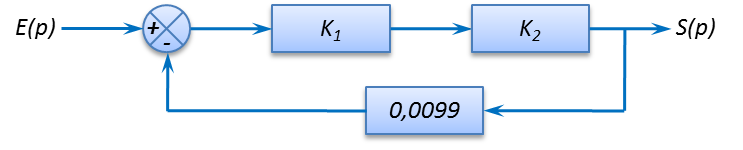
\includegraphics[width=0.7\textwidth]{png/fig_01}\\
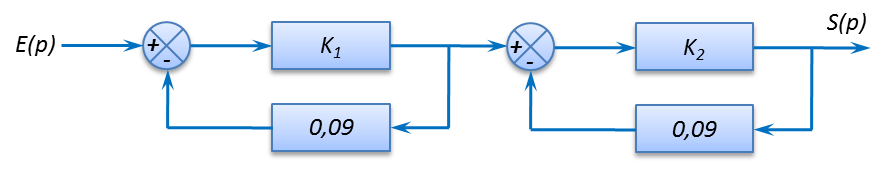
\includegraphics[width=0.7\textwidth]{png/fig_02}
\end{center}


\vspace{.5cm}

Le premier système a pour fonction de transfert $H_1(p)$ et le deuxième $H_2(p)$. 

\subsubsection{Travail demandé}
\begin{enumerate}
\item Calculer $H_1(p)$ et $H_2(p)$.
\item On pose $K_1=K_2=K$. Calculer $K$ tel que $H_1(p)=H_2(p)$.
\end{enumerate}

\correction{
\begin{enumerate}
\item Dans le premier cas, on peut calculer la fonction de transfert en boucle fermée :
$$
H_1(p)=\dfrac{S(p)}{E(p)}=\dfrac{K_1(p)K_2(p)}{1+K_1(p)K_2(p) K_3}
$$

Dans le second cas, deux FTBF se succèdent. On a :
$$
H_2(p)=\dfrac{S(p)}{E(p)}=\dfrac{K_1(p)}{1+K_1(p) K_4}\cdot \dfrac{K_2(p)}{1+K_2(p) K_3}
= \dfrac{K_1(p) K_2(p)}{\left(1+K_1(p)K_4\right)\cdot\left(1+K_2(p)K_4\right)}
$$
\item Dans le premier cas :
$$
H_1(p) = \dfrac{K^2}{1+K^2 K_3}
$$

Dans le second cas :
$$
H_2(p)= \dfrac{K^2}{\left(1+KK_4\right)\cdot\left(1+KK_4\right)}
= \dfrac{K^2}{ 1+K^2K_4^2+2KK_4}
$$

Ainsi,
$$
H_1(p)=H_2(p) 
\Longleftrightarrow 
\dfrac{K^2}{1+K^2 K_3}= \dfrac{K^2}{ 1+K^2K_4^2+2KK_4}
\Longleftrightarrow 
\dfrac{1}{1+K^2 K_3}= \dfrac{1}{ 1+K^2K_4^2+2KK_4}
$$

$$
\Longleftrightarrow 
1+K^2 K_3 = 1+K^2K_4^2+2KK_4
\Longleftrightarrow 
K K_3 = KK_4^2+2K_4
\Longleftrightarrow 
K = \dfrac{2K_4}{K_3-K_4^2} = 100
$$
\end{enumerate}
}
\newpage

%--------------------------------------------

\exercice{Schémas blocs élémentaires}

On considère le système suivant : 
\begin{center}
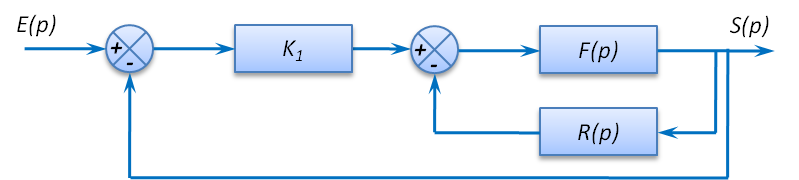
\includegraphics[width=.7\textwidth]{png/fig_03}
\end{center}

\subsubsection{Travail demandé}
\begin{enumerate}
\item Calculer la fonction de transfert $H(p)$ du système.
On donne pour valeur aux différents blocs $F(p)=\dfrac{8}{p\left(p+4 \right)\left( p+5\right)}$, $R(p)=p$ et $K_1 = 5$.
\item Calculer $H(p)$.
\end{enumerate}


\correction{
\begin{enumerate}
\item Schéma bloc équivalent :
\begin{center}
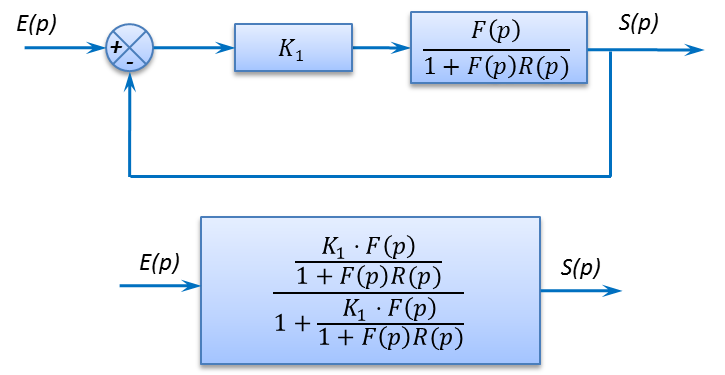
\includegraphics[width=.6\textwidth]{png/fig_03_Corr}
\end{center}

$$
\dfrac{S(p)}{E(p)} = \dfrac{K_1 F(p)}{1+F(p)R(p)+K_1 F(p)}
$$
\item On remplace les fonctions de transfert par leurs valeurs : 
$$
\dfrac{S(p)}{E(p)} = \dfrac{K_1 \dfrac{8}{p\left(p+4 \right)\left( p+5\right)}}{1+\dfrac{8p}{p\left(p+4 \right)\left( p+5\right)}+K_1 \dfrac{8}{p\left(p+4 \right)\left( p+5\right)}}
= \dfrac{8 K_1}{p\left(p+4 \right)\left( p+5\right)+8p+8 K_1 }
$$
\end{enumerate}
}
\newpage

%--------------------------------------------

\exercice{Schémas blocs élémentaires}

Déterminer la sortie $S(p)$ et éventuellement la fonction de transfert correspondant aux schémas suivants : 

\begin{enumerate}
\item Premier système
\begin{center}
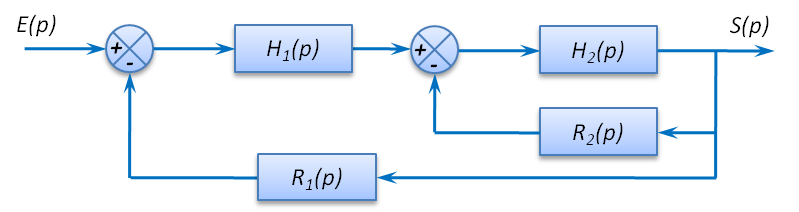
\includegraphics[width=.7\textwidth]{png/fig_04}
\end{center}
\item Deuxième système
\begin{center}
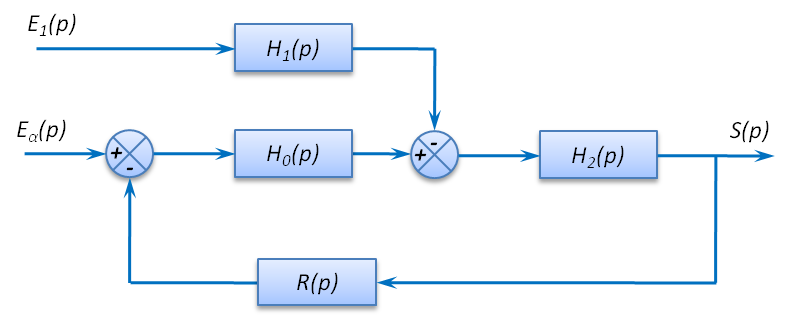
\includegraphics[width=.7\textwidth]{png/fig_05}
\end{center}
\item Troisième système
\begin{center}
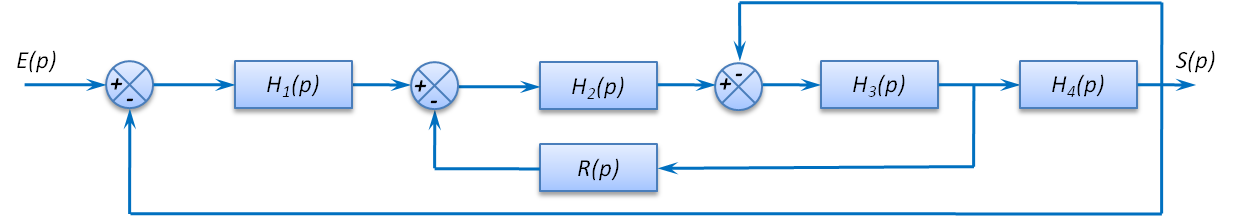
\includegraphics[width=\textwidth]{png/fig_06}
\end{center}
\end{enumerate}

\correction{
\begin{enumerate}
\item Premier système
\begin{center}
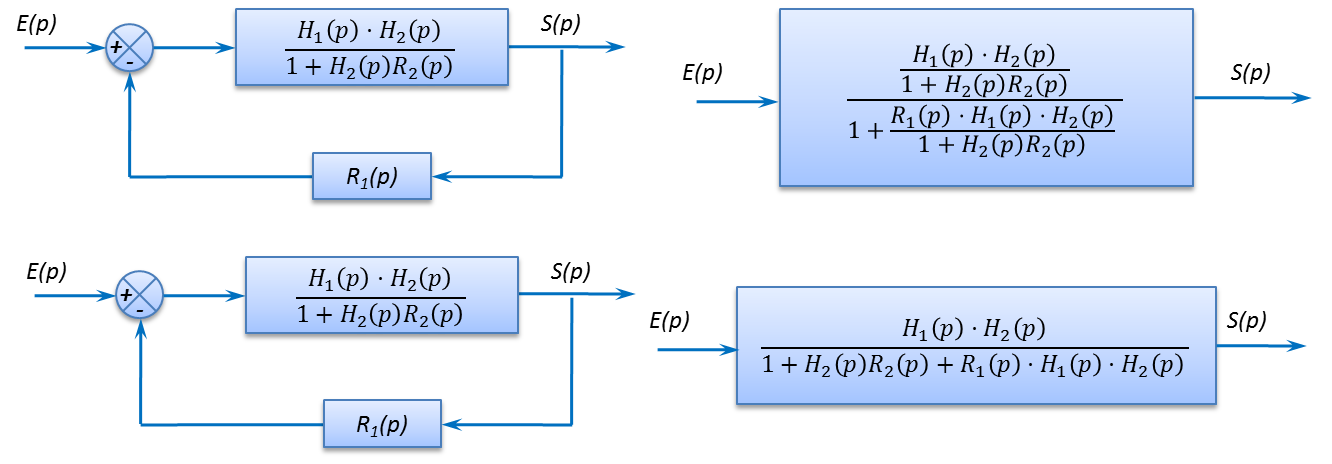
\includegraphics[width=.9\textwidth]{png/fig_04_Corr}
\end{center}
\item Deuxième système\\
On note $G_1(p)=\dfrac{S(p)}{E_\alpha (p)}$ lorsque $E_1(p)=0$ : 
$$
G_1(p)=\dfrac{H_0(p)\cdot H_2(p)}{1+H_0(p)\cdot H_2(p)\cdot R(p)}
$$

On note $G_2(p)=\dfrac{S(p)}{E_1(p)}$ lorsque $E_{\alpha}(p)=0$ :
$$
G_2(p)=-H_1(p)\cdot \dfrac{H_2(p)}{1+H_0(p)\cdot H_2(p)\cdot R(p)}
$$

Au final, 
$$
S(p)=G_1(p)E_{\alpha}(p) + G_2(p) E_1(p)
$$
\item Troisième système
\begin{center}
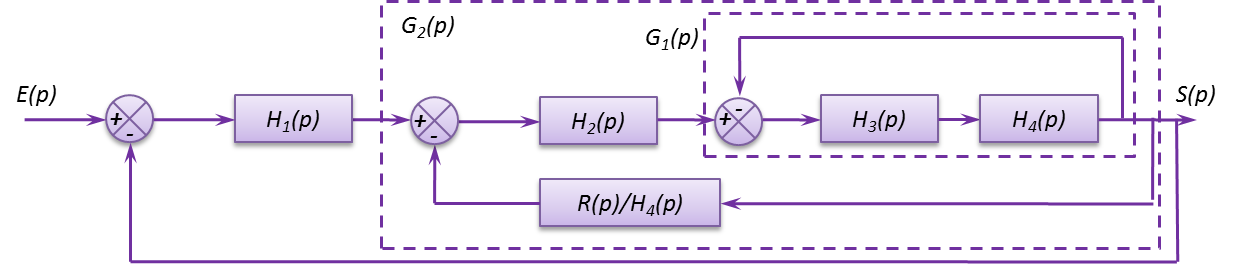
\includegraphics[width=.9\textwidth]{png/fig_06_Corr}
\end{center}
On a :
$$
G_1(p)=\dfrac{H_3(p)\cdot H_4(p)}{1+H_3(p)\cdot H_4(p)}
$$

\begin{align*}
G_2(p) &= 
\dfrac{H_2(p)\cdot G_1(p)}{1+H_2(p)\cdot G_1(p)\cdot\dfrac{R(p)}{H_4(p)}}
= 
\dfrac{H_2(p)\cdot \dfrac{H_3(p)\cdot H_4(p)}{1+H_3(p)\cdot H_4(p)}}{1+H_2(p)\cdot \dfrac{H_3(p)\cdot H_4(p)}{1+H_3(p)\cdot H_4(p)}\cdot\dfrac{R(p)}{H_4(p)}}\\
&= 
\dfrac{H_2(p)\cdot H_3(p)\cdot H_4(p)}{1+H_3(p)\cdot H_4(p)+H_2(p)\cdot H_3(p)\cdot R(p)}
\end{align*}

Au final, 
$$
H(p)=\dfrac{H_1(p)\cdot G_2(p)}{1+H_1(p)\cdot G_2(p)}
=
\dfrac{H_1(p)\cdot \dfrac{H_2(p)\cdot H_3(p)\cdot H_4(p)}{1+H_3(p)\cdot H_4(p)+H_2(p)\cdot H_3(p)\cdot R(p)}}{1+H_1(p)\cdot \dfrac{H_2(p)\cdot H_3(p)\cdot H_4(p)}{1+H_3(p)\cdot H_4(p)+H_2(p)\cdot H_3(p)\cdot R(p)}}
$$
$$
H(p)=
\dfrac{H_1(p)\cdot H_2(p)\cdot H_3(p)\cdot H_4(p)}{1+H_3(p)\cdot H_4(p)+H_2(p)\cdot H_3(p)\cdot R(p)+H_1(p)\cdot H_2(p)\cdot H_3(p)\cdot H_4(p)}
$$
\end{enumerate}
}
\newpage

%--------------------------------------------

\exercice{Schémas blocs élémentaires}
D\'eterminez la fonction de transfert, $H(p)= \frac{S}{E}$, des schémas blocs suivant :
\begin{itemize}
\item Sch\'ema bloc $1$ :
\begin{center}
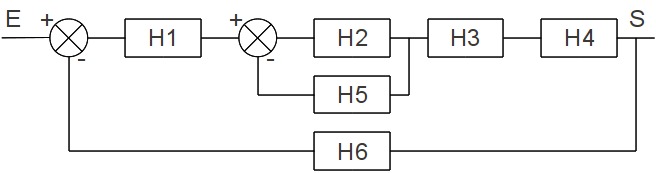
\includegraphics[scale=0.8]{png/schemabloc1.png}
\end{center}
\item Sch\'ema bloc $2$ :
\begin{center}
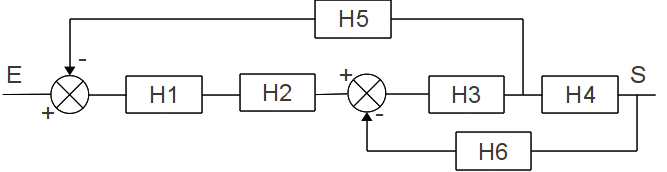
\includegraphics[scale=0.8]{png/schemabloc2.png}
\end{center}
\end{itemize}

\correction{ % Answer
\begin{itemize}
\item Schéma bloc $1$ : \[\frac{S}{E}=\frac{\frac{H_1H_2H_3H_4}{1+H_2H_5}}{1+\frac{H_1H_2H_3H_4H_6}{1+H_2H_5}}\]
\item Schéma bloc $2$ : \[\frac{S}{E}=\frac{H_1H_2H_3H_4}{1+H_3(H_4H_6+H_1H_2H_5)}\]
\end{itemize}
}
\newpage

%--------------------------------------------

\exercice{Système asservi}
D\'eterminez la fonction de transfert, $H(p)= \frac{S(p)}{E(p)}$, du schéma bloc suivant :

\begin{center}
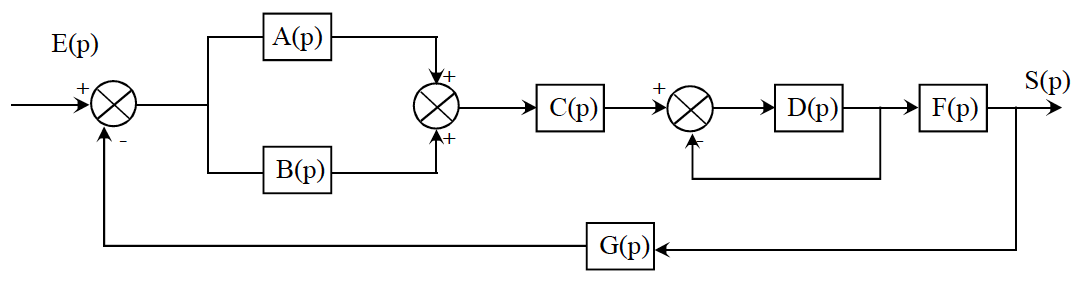
\includegraphics[scale=0.4]{png/SB3.png}
\end{center}

\textit{Remarque : pour alléger l'écriture des calculs, on pourra noter $A$, $B$, $C$\dots les fonctions $A(p)$, $B(p)$, $C(p)$\dots}

\correction{ % Answer
\[\frac{S}{E}=\frac{(A+B).C.D.F}{1+D+(A+B).C.D.F.G}\]
}
\newpage

%--------------------------------------------

\exercice{Moteur à courant continu}
Considérons un moteur à courant continu ayant pour modèle de connaissance les équations suivantes :

\begin{center}
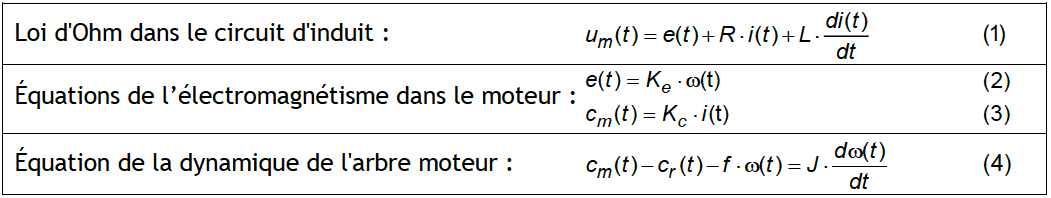
\includegraphics[scale=0.4]{png/MCC_data1.png}
\end{center}

avec :

\begin{center}
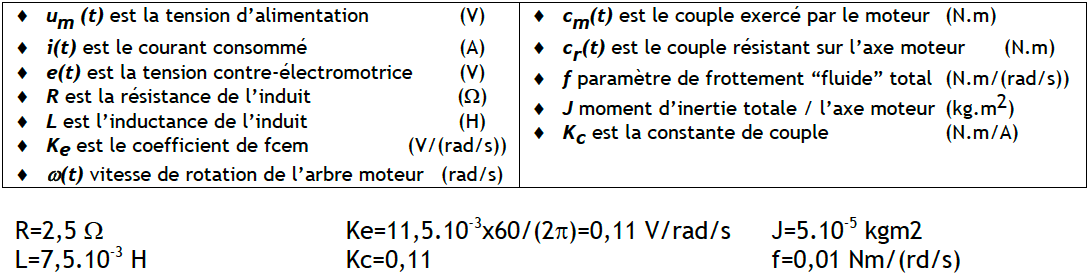
\includegraphics[scale=0.4]{png/MCC_data2.png}
\end{center}

\subsubsection{Travail demandé}
\begin{enumerate}
\item Les conditions initiales étant nulles, compléter le shéma-bloc ci-dessous dans le domaine de Laplace.
\begin{center}
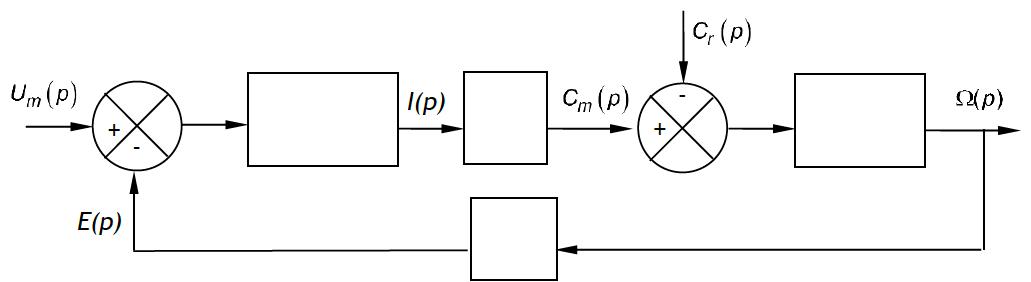
\includegraphics[scale=0.4]{png/MCC_bloc.png}
\end{center}
\item Ce shéma comporte une boucle et des comparateurs. Est-ce un système asservi ?
\item Exprimer de façon littérale la fonction de transfert $\frac{\Omega(p)}{U_m(p)}$ pour $C_r(p)=0$ (sans perturbation).
\item Exprimer de façon littérale la fonction de transfert $\frac{\Omega(p)}{C_r(p)}$ pour $U_m(p)=0$.
\item En précisant le théorème utilisé, en déduire l'expression de $\Omega(p)$ en fonction de $U_m(p)$ et $C_r(p)$.
\item Donner l'expression de $\omega(t=+\infty)$ lorsque $u_m(t)=U_{m0}$ (constante) et $c_r(t)=C_{r0}$ (constante).
\item Vérifier que $K_c.U_{m0}$ et $R.C_{r0}$ sont de même dimension ainsi que $R.f$ et $K_e.K_c$.
\item Faire l'application numérique pour les deux valeurs de $C_{r0}$ ($0$ et $0,3 N.m$) et pour $U_{m0}=10V$.
\item Ces résultats sont-ils cohérents avec la courbe ci-dessous obtenue par simulation numérique ?
\begin{center}
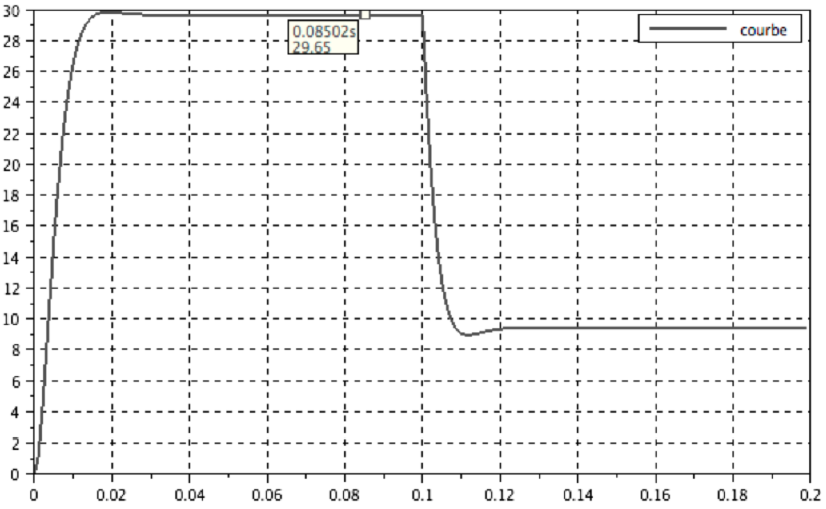
\includegraphics[scale=0.5]{png/MCC_releves.png}
\end{center}
\end{enumerate}

\correction{ % Answer
\begin{enumerate}
\item Schéma bloc :
\begin{center}
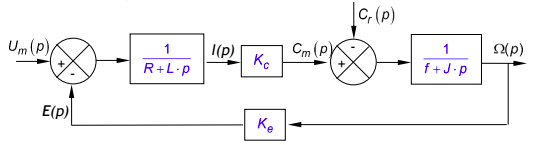
\includegraphics[scale=0.7]{png/MCC_bloc-cor.png}
\end{center}
\item NON. La grandeur de sortie n'est pas de même nature que la grandeur d'entrée. Il n'y a pas de capteur. Le schéma représente la structure des équations différentielles du modèle de connaissances, pas un système asservi.
\item Avec $C_r(p)=0$ :
\[\frac{\Omega(p)}{U_m(p)}=(\frac{K_c}{R.f+K_e.K_c}).(\frac{1}{1+\frac{R.J+L.f}{R.f+K_e.K_c}p+\frac{L.J}{R.f+K_e.K_c}p^2})=F_1(p) \]
\item Avec $U_m(p)=0$ :
\[\frac{\Omega(p)}{U_m(p)}=(\frac{-R}{R.f+K_e.K_c}).(\frac{1+\frac{L}{R}p}{1+\frac{R.J+L.f}{R.f+K_e.K_c}p+\frac{L.J}{R.f+K_e.K_c}p^2})=F_2(p) \]
\item Si $C_r(p)$ et $U_m(p)$ sont non nulles alors : $\Omega(p)=F_1(p)U_m(p)+F_2(p)C_r(p)$ (Théorème de superposition)
\item \[\omega(+\infty)=\lim_{t \leftrightarrow 0}p\Omega(p)=\frac{K_c.U_m{m0}-R.C_{r0}}{R.f+K_e.K_c} \]
\item Cf. dimensions données dans l'énoncé
\item AN : $\omega(+\infty)=29,6 rad/s$ pour $C_{r0}=0$ et  $\omega(+\infty)=9,4 rad/s$ pour $C_{r0}=0,3$.
\item Ces résultats sont similaires à ceux obtenu par simulation. Ce qui est cohérent puisque la simulation ne fait que résoudre numériquement les mêmes équations du modèles de connaissance.
\end{enumerate}
}
\newpage

%--------------------------------------------


%----------------------------------------------------------------------------------------
%	Fonctions de transfert du 1er ordre
%----------------------------------------------------------------------------------------
\section{Fonctions de transfert du 1er ordre}

%--------------------------------------------
\exercice{Identification des systèmes d'ordre 1}

\begin{enumerate}
\item Pour chacune des courbes suivantes, donner l'expression de la fonction de transfert.
\end{enumerate}

\begin{minipage}[c]{.49\linewidth}
\begin{center}
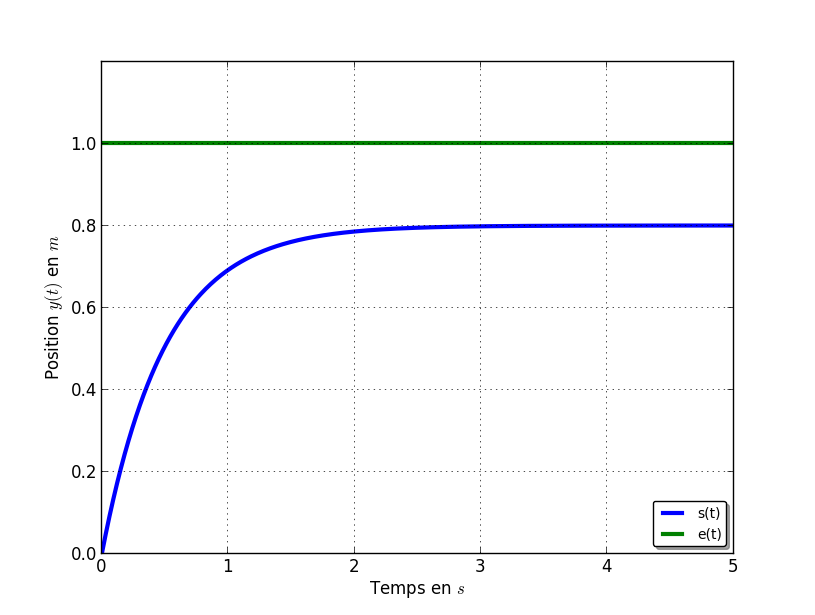
\includegraphics[width=\textwidth]{png/courbe1-1O}
\end{center}
\end{minipage}\hfill
\begin{minipage}[c]{.49\linewidth}
\begin{center}
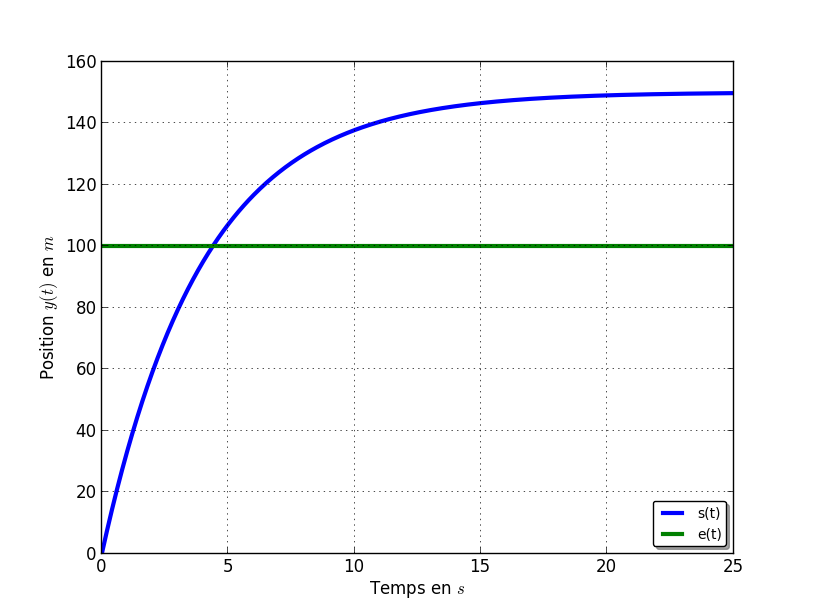
\includegraphics[width=\textwidth]{png/courbe2-1O}
\end{center}
\end{minipage}

\begin{minipage}[c]{.49\linewidth}
\begin{center}
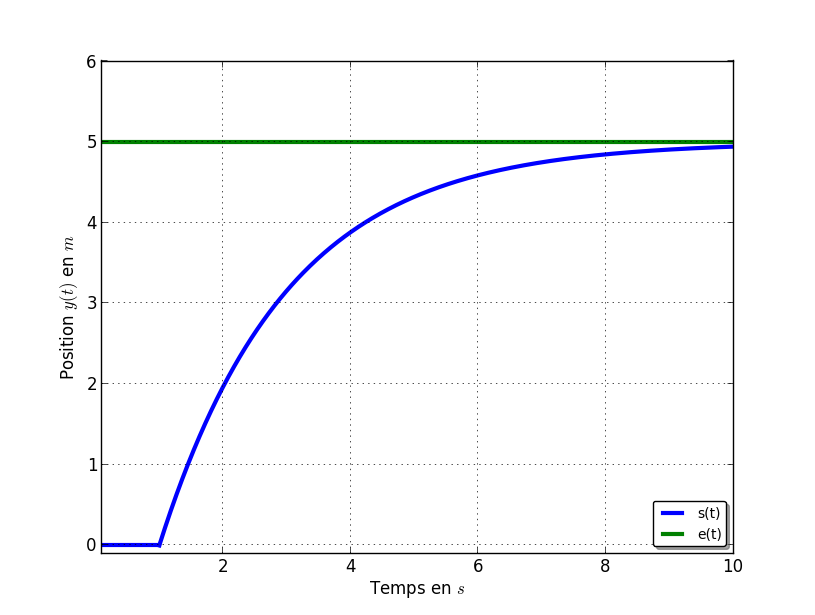
\includegraphics[width=\textwidth]{png/courbe3-1O}
\end{center}
\end{minipage}\hfill
\begin{minipage}[c]{.49\linewidth}
\begin{center}
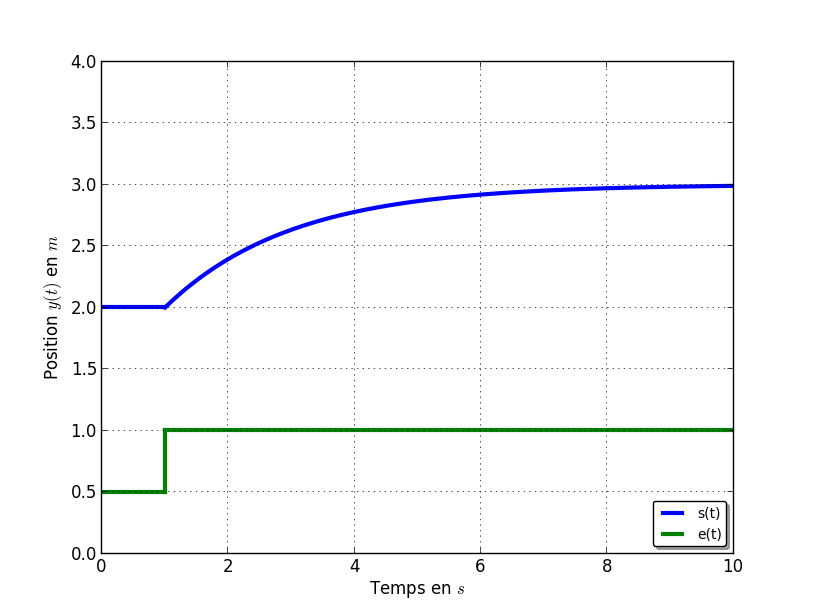
\includegraphics[width=\textwidth]{png/courbe4-1O}
\end{center}
\end{minipage}
\newpage

%--------------------------------------------
\exercice{Étude des performances du système d'ouverture de porte automatique de TGV}
\begin{minipage}[c]{.45\linewidth}
\begin{center}
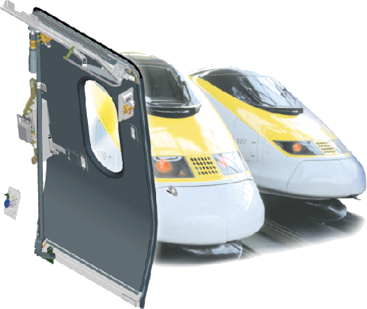
\includegraphics[width=.6\textwidth]{png/fig_01-TGV}
\end{center}
 
 La figure de droite montre l’interface assurant, à partir des informations délivrées par l’unité centrale de commande, la fermeture hermétique et le verrouillage d’une porte de TGV. 
 
\end{minipage} \hfill
\begin{minipage}[c]{.52\linewidth}
\begin{center}
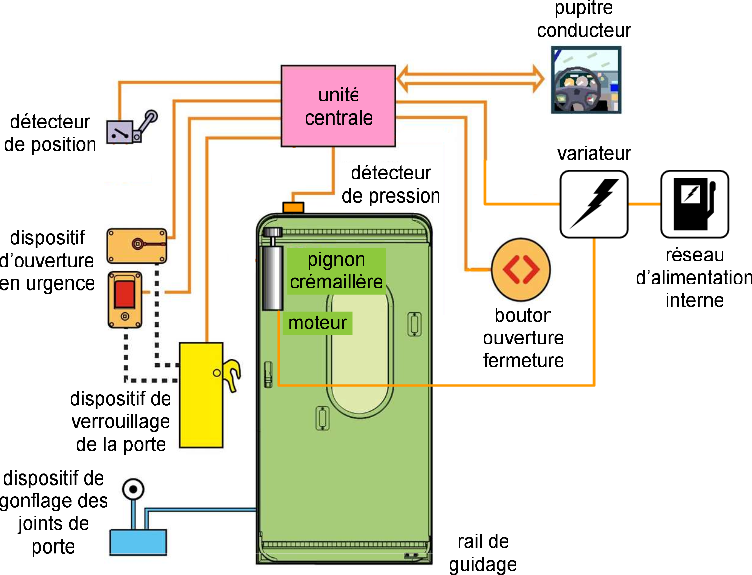
\includegraphics[width=\textwidth]{png/fig_02-TGV}
\end{center}
\end{minipage}

\begin{minipage}[c]{.6\linewidth}
Afin de satisfaire les contraintes d'encombrement, l'ouverture de la porte s'effectue selon l'enchaînement temporel de trois phases distinctes décrites à partir de la position « porte fermée » pour laquelle la face extérieure de la porte est alignée avec la face extérieure de la caisse : une phase de décalage puis une phase de louvoiement et enfin une phase d'escamotage. La phase primaire (décalage) puis la phase terminale (escamotage) sont définies par les figures ci-contre. 

\end{minipage} \hfill
\begin{minipage}[c]{.35\linewidth}
\begin{center}
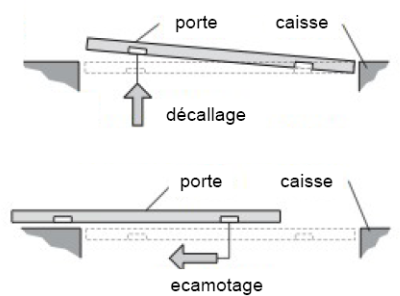
\includegraphics[width=\textwidth]{png/fig_03-TGV}
\end{center}
\end{minipage}

\vspace{0.5cm}
Les performances annoncées de la part du constructeur, dans la phase d'escamotage, sont les suivantes :
\vspace{0.5cm}
\begin{center}
\begin{tabular}{|l|l|}
\hline
Critères & Valeur \\
\hline
\hline
Accès suffisant du wagon & 850 mm \\
\hline
Temps d'ouverture de la porte en phase d'escamotage & $t\leq 4\; s$ \\
\hline
Vitesse d’accostage de la porte en fin de phase d’escamotage & $V\leq 0,09 \; m/s$ \\
\hline
\end{tabular}
\end{center}
\vspace{0.5cm}

Pour ouvrir la porte, on utilise un moteur, dont la rotation est transformée en translation par l'intermédiaire d'un système pignon crémaillère. La translation de la porte est notée $y(t)$. L'angle de rotation du moteur est noté $\theta_m(t)$. Le lien entre $y(t)$ et $\theta_m (t)$ est $y(t) = R\cdot\theta_m (t)$ où $R$ est le rayon du pignon ($R=37\; mm$).

On fait l'hypothèse qu'à l'instant initial, correspondant au début de la translation de la porte, la porte est immobile, avec $y(t=0)=0$ et $\theta_m (t=0)=0$ (toutes les autres conditions initiales seront également nulles, par conséquent).

Grâce à une redéfinition du paramétrage et dans un souci de simplification, on considère qu'au cours de cette d phase la vitesse angulaire du moteur vérifie $\omega_m (t) = \dot{\theta}_m (t) \geq 0$ et la position de la porte vérifie $y(t) \geq 0$.  


On donne le modèle de connaissance du moteur courant continu du système :
$$u_m(t) = e(t) + R\cdot i(t) 
\quad e(t) = k\cdot \omega_m(t) 
\quad J\cdot \dfrac{d\omega_m(t)}{dt} = C_m (t)
\quad C_m (t) = k_m \cdot i(t)$$

\vspace{0.5cm}
Avec : 
\begin{itemize}
\item $u_m (t)$ : tension du moteur; 
\item $e(t)$ : force contre électromotrice du moteur; 
\item $i(t)$ :intensité dans le moteur;
\item $C_m (t)$ : couple exercé par le moteur;
\item $\omega_m(t)$ : vitesse angulaire du moteur.
\end{itemize}

\subsubsection{Travail demandé}
\begin{enumerate}
\item Exprimer ces équations dans le domaine de Laplace.
\item Schématiser le schéma-bloc du moteur en s’aidant des équations de la question 1.
\item Montrer que, dans le domaine de Laplace, la relation entre $\Omega_m (p)$ et $U_m (p)$ peut s'écrire sous la forme : $\dfrac{\Omega_m(p)}{U_m(p)} = \dfrac{K}{1+Tp} $ où $K$ et $T$ sont deux constantes à déterminer.
\item Déterminer $\omega_m (t)$ lorsque le moteur est soumis à un échelon de tension d'amplitude $u_0$ tel que : $u_m (t)= u_0 \cdot u(t)$. Exprimer et justifier le résultat en fonction de $K$ et $T$.
\item L'application numérique fournit $K=1,2 \; s^{-1}\cdot V^{-1}$ et $T=0,16\;s$. Déterminer le temps de réponse à 5\% du moteur.\\
Le schéma bloc du système peut se mettre sous la forme suivante :
\begin{center}
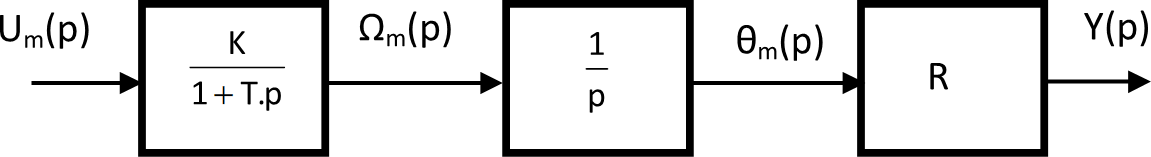
\includegraphics[width=.5\textwidth]{png/fig_04-TGV}
\end{center} 
\item Justifier la fonction de transfert entre $\Omega_m(p)$ et $\theta_m (p)$.
\item Déterminer l'expression analytique de $\dfrac{Y(p)}{U_m(p)}$.
\item Déterminer l'expression analytique de $y(t)$ lorsque le moteur est soumis à un échelon de tension d'amplitude $u_0$.
\item Déterminer la valeur numérique du déplacement de la porte au bout de 4s ($u_0 =5V$), et conclure quant à la capacité du système à satisfaire le critère d'accès au wagon du cahier des charges.
\item Déterminer la vitesse de la porte à la fin de la translation ($v(t=4s)= \dfrac{d}{dt}y(t=4s)$). Conclure quant à la capacité du système à satisfaire le critère de vitesse finale de translation de la porte du cahier des charges.
\end{enumerate}
\newpage

%--------------------------------------------
\exercice{Robot de manutention}

\subsubsection{Présentation}

Dans ce qui suivra on se placera dans l’hypothèse de systèmes linéaires continus et invariants.


\begin{minipage}[c]{.3\linewidth}
\begin{center}
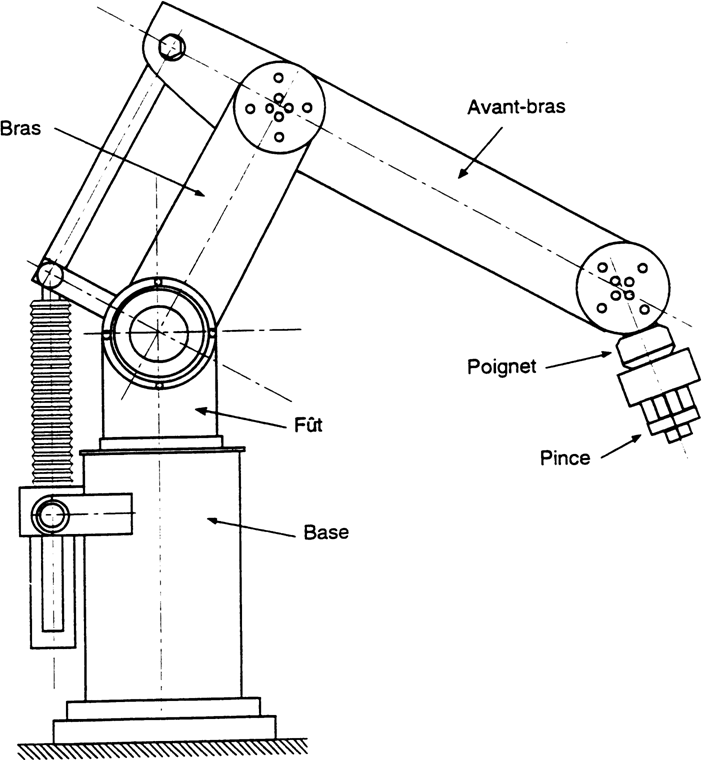
\includegraphics[width=\textwidth]{png/fig_01-1O}
\end{center}
\end{minipage} \hfill
\begin{minipage}[c]{.65\linewidth}
Principales notations utilisées : 
\begin{itemize}
\item $J_m$ : inertie du moteur, du réducteur et de la charge;
\item $J_{me}$ : inertie globale équivalente sur l’arbre moteur;
\item $C_m$ : couple électromagnétique délivré par le moteur;
\item $C_{re}$ : couple résistant ramené sur l’arbre moteur ou couple équivalent;
\item $R$, $Ke$, $Kt$ : constantes électriques du moteur (résistance de l’induit, constante 	de force contre électromotrice et constante de couple);
\item $N$ : rapport de réduction;
\item $\omega_m$, $\theta_m$ : vitesse et position angulaire du moteur;
\item $\omega_c$, $\theta_c$ : vitesse et position angulaire de la charge.
\end{itemize}
\end{minipage}

On se propose tout d’abord d’étudier le modèle du moteur à vide c’est à dire du moteur seul : dans un premier temps par un modèle théorique et dans un second temps par une étude expérimentale. Ensuite il sera fait mention de la charge puis de la réalisation de l’asservissement de position.

\subsubsection{Étude théorique du moteur seul}

Le moteur retenu pour animer la rotation du fût par rapport à la base est un servomoteur PARVEX de type AXEM à induit plat qui présente l’avantage de posséder une très faible inertie. C’est un moteur à courant continu.

Le comportement électromécanique de ce moteur dans l’hypothèse où l’inductance est négligeable, est donné par les équations suivantes :

\begin{eqnarray*}
u(t)=Ri(t)+e(t) \\
C_m(t)=K_t i(t) \\
e(t)= K_e \omega_m(t) \\
J_m \dfrac{d\omega_m (t)}{dt} = C_m(t)
\end{eqnarray*}


\begin{enumerate}
\item En faisant l’hypothèse de conditions initiales sont nulles, calculez la transformée de Laplace $\Omega(m)$ en fonction de la transformée de Laplace $U(p)$.
\item Mettez le résultat sous la forme $\Omega_m(p)=\dfrac{K_m}{1+T_m p} U_m(p)$ en précisant $K_m$ et $T_m$.
\item Les données du constructeur permettent de connaître les valeurs suivantes : $K_e=25,5\; V/(1000\; tr/min))$, $K_t=0,244 \; Nm/A$, $R=0,46\, \Omega$.\\
Faites un calcul approché permettant de déterminer $K_m$ et $T_m$ ($T_m$  sera fonction de $J_m$  pour l’instant non connu).\\
\textit{Remarque : pour toutes les applications numériques utilisez des unités S.I.}
\end{enumerate}

\subsubsection{Étude pratique du moteur seul}

Afin de valider le modèle précédent et de déterminer l’inertie du rotor du moteur on effectue une étude expérimentale sous la forme de l’observation de la réponse du moteur seul soumis à un échelon de tension de 50 V. Le résultat de cet essai est donné sur la courbe suivante.

\begin{center}
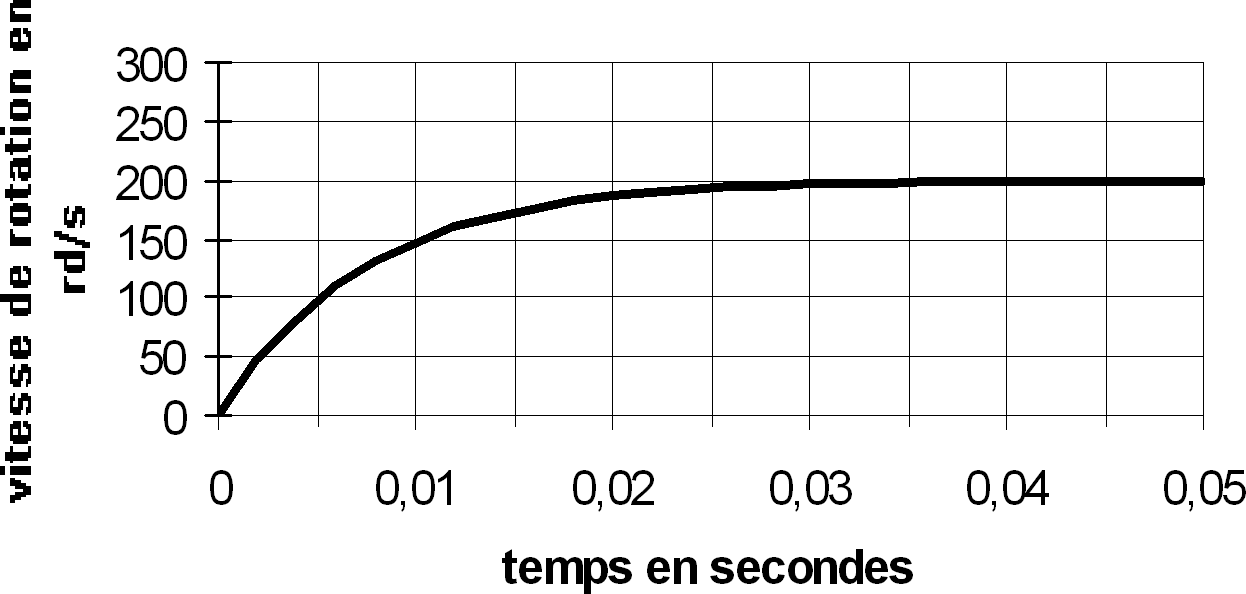
\includegraphics[width=.5\textwidth]{png/fig_02-1O}
\end{center}

\begin{enumerate}
\item Cette courbe est-elle bien conforme au modèle du premier ordre de la question précédente ? Pourquoi ?
\item Déterminez les valeurs expérimentales de $K_m$ et $T_m$. Déduisez-en la valeur expérimentale de $J_m$.
\end{enumerate}

\subsubsection{Motorisation complète avec réducteur et charge}

La charge que devra entraîner le moteur est maintenant prise en compte ainsi que le réducteur qui permet de réduire la vitesse $\omega_m$ de rotation du moteur. En sortie du réducteur la vitesse de rotation est $\omega_c$.

L’inertie du moteur seule $J_m$ devient $J_{me}$ inertie équivalente de l’ensemble  charge + moteur + réducteur.

La charge crée un couple résistant équivalent $C_{re}$. On obtient donc l’équation suivante :
$$
C_m(t)=J_{me}\dfrac{d\omega_m(t)}{dt} + C_{re}(t)
$$

\begin{enumerate}
\item A partir des équations électriques du moteur et de l’équation précédente, exprimez la transformée $\Omega_m(p)$. Les dénominateurs seront mis sous la forme $(1+T_{me} p)$. On précisera l’expression de $T_{me}$.
\item A partir du résultat précédent complétez le schéma fonctionnel suivant et explicitez clairement $G_1$, $G_2$, $G_3$, $G_4$. $G_3$ sera exprimé sous la forme d’un premier ordre avec pour constante de temps $T_{me}$.
\end{enumerate}

\begin{center}
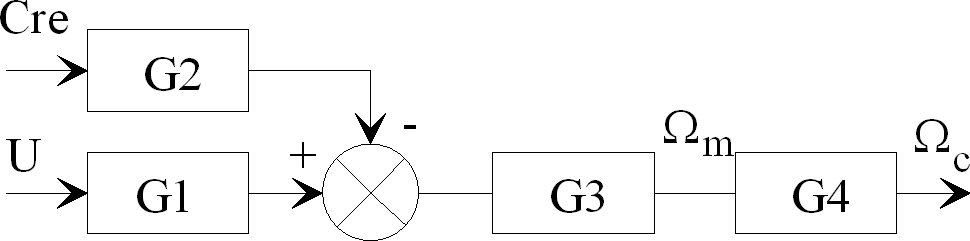
\includegraphics[width=0.5\textwidth]{png/fig_03-1O}
\end{center}

\subsubsection{Asservissement de position}

Pour la suite on suppose $C_{re}(p)$  nul. 

 Pour assurer l’asservissement de position angulaire du fût du robot (la sortie est alors un angle exprimé en radian), on associe au moteur un variateur de gain pur $K_a$ placé avant $G_1$ et on met en place un capteur de position angulaire de gain unitaire. Le capteur prendra l’information de position après le réducteur.
 
\begin{enumerate}
\item Faites le schéma fonctionnel de l’asservissement ainsi constitué.
\item Calculez sa fonction de transfert. Donnez-en une interprétation pratique.
\end{enumerate}
\newpage

%----------------------------------------------------------------------------------------
%	Fonctions de transfert du 2ème ordre
%----------------------------------------------------------------------------------------
\section{Fonctions de transfert du 2ème ordre}

%--------------------------------------------
\exercice{Correcteur de phare}
\textit{(Selon le concours CCP PSI 2003)}

\subsubsection{Présentation du système}

L‘assiette d‘un véhicule se modifie avec sa charge, le profil de la route ou les
conditions de conduite (phase de freinage ou d‘accélération). Cette modification
entraîne une variation d‘inclinaison de l‘axe du faisceau lumineux produit par
les phares du véhicule. Ceux ci peuvent alors éblouir d‘autres conducteurs ou
mal éclairer la chaussée.


\begin{center}
 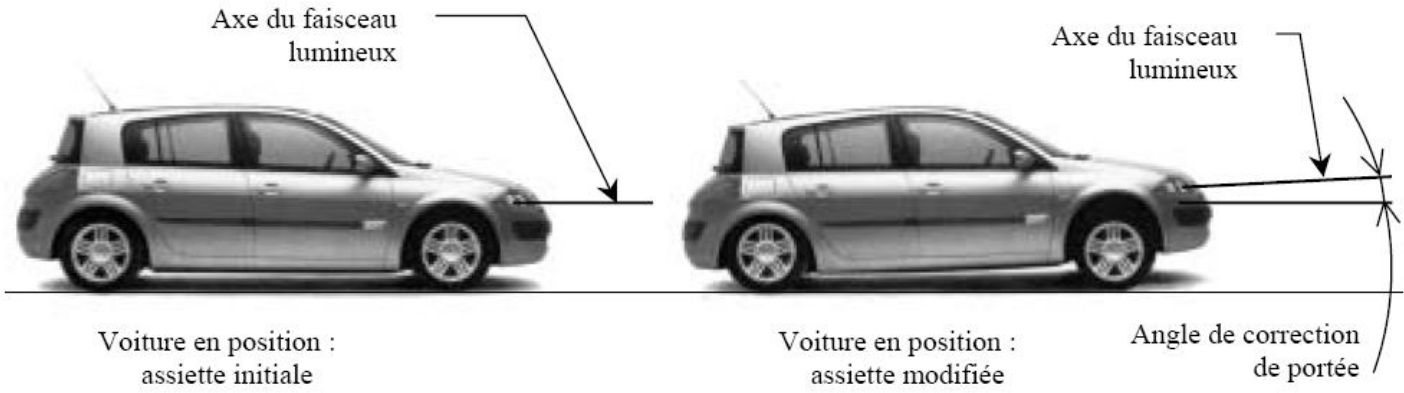
\includegraphics[width=.6\textwidth]{png/image1}
\end{center}
     
         Certaines voitures sont équipées de système de correction de portée. Ce
système fait appel à
des capteurs d‘assiette reliés aux essieux avant et arrière du véhicule. Les
données sont traitées
électroniquement par un calculateur et transmises aux actionneurs situés
derrière les projecteurs. La
position du projecteur est ajustée en maintenant un angle de faisceau optimal
évitant tout
éblouissement et fournissant le meilleur éclairage de la route.
Le système étudié est un correcteur de portée statique, qui corrige la portée
lorsque le véhicule est à
l‘arrêt et conserve cette correction lorsque le véhicule roule (le correcteur ne
tient compte que de la
variation d‘assiette due à la charge).

       Le but de l‘étude est d‘analyser le système et de montrer s‘il est
capable de corriger la portée
de manière dynamique, c‘est à dire en tenant compte des variations d‘assiette
dues au profil de la
route.

\subsubsection{Éléments constitutifs du correcteur de portée}

\textbf{Capteurs d’assiette} : codeurs optiques permettant de mesurer le
débattement des suspensions.

\textbf{Système d’orientation : bloc d’orientation + moto-réducteur + système
vis écrou}

Le bloc d‘orientation supporte les différentes lampes du phare (codes,
clignotants...). Il peut pivoter
par rapport au support lié à la carrosserie autour d‘un axe horizontal (axe de
rotation indiqué sur la
figure ci-dessous). Le bloc est protégé par une vitre liée à la carrosserie. Ce
mouvement est motorisé
grâce au moto-réducteur + système vis écrou. Il existe aussi une possibilité de
réglage manuel en
sortie d‘usine ou en cas de défaillance du système électrique.

\begin{center}
 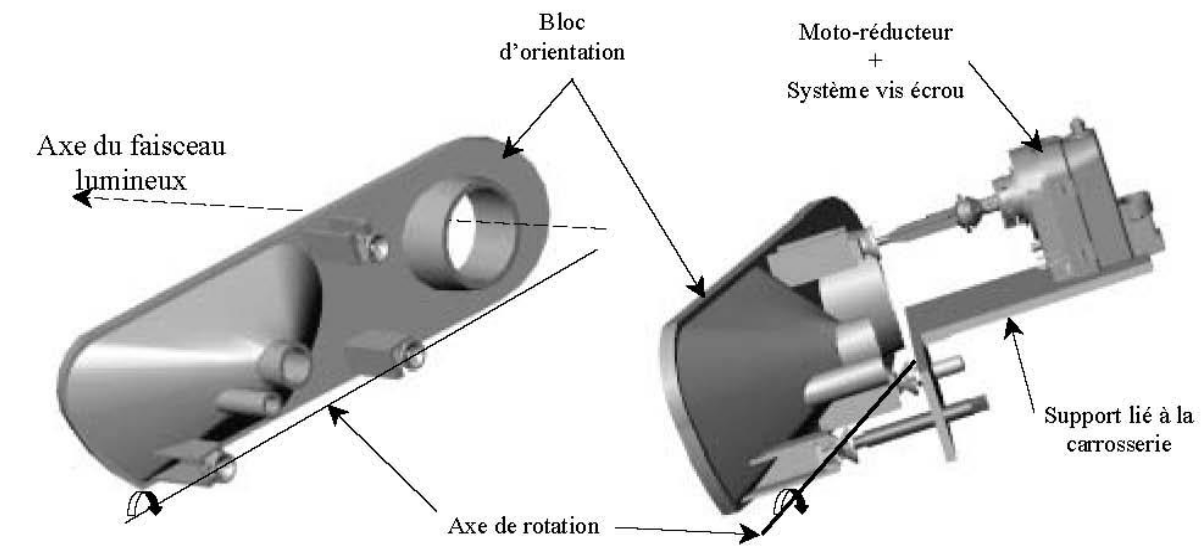
\includegraphics[width=.6\textwidth]{png/image2}
\end{center}

\subsubsection{Diagrammes SADT niveau A-0, A0 et A3}
\begin{center}
 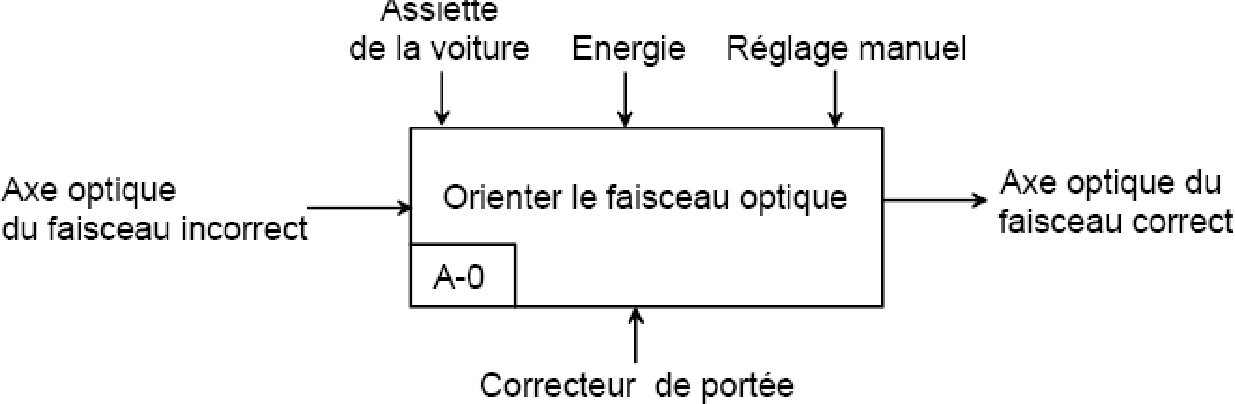
\includegraphics[width=.6\textwidth]{png/image3}
\end{center}

\subsubsection{Étude de la chaîne d’action complète}
La chaîne d‘action complète comprend :
\begin{itemize}
 \item l‘ensemble transducteur (\textbf{capteur + amplificateur + calculateur})
qui mesure l‘angle de tangage $\beta$ du véhicule et commande le moteur du
système. L‘ensemble est assimilable à un gain pur : $K_c$;
\item le \textbf{moteur à courant continu} dont la fonction de transfert est
notée $M(p)$;
\item on équipe ce moteur d‘un retour tachymétrique assimilable à un gain pur : 
   $K_{tachy}=0,03 V.rad^{-1}.s$;
\item le \textbf{réducteur de vitesse} dont le rapport de réduction est de 490;
\item l’ensemble \textbf{vis-écrou} (de pas $p = 6mm$) qui transforme la
rotation de l’axe du réducteur en translation de l’axe de sortie. (NB : 1
tour de la vis fait avancer de 1 pas l’écrou);
\item le \textbf{bloc d‘orientation} : l‘angle de correction de portée
$\theta(t)$ étant petit, on peut linéariser la loi entrée-sortie sur le
domaine d‘utilisation ; l‘angle $\theta(t)$ est proportionnel au déplacement
$x(t)$ de la vis.
\end{itemize}

($\theta(t)$ varie entre $\dfrac{-\pi}{20}$ $\dfrac{\pi}{20}$ et pour
$x(t)$ compris entre -15mm et +15mm).

\begin{enumerate}

\item Refaire, sur votre copie, le diagramme fonctionnel de la chaîne d‘action
ci-dessous, en précisant le nom des constituants dans les blocs, les
informations véhiculées entre les blocs ainsi que leur symbole et leur unité
(les fonctions de transfert ne seront pas déterminées).\\
NB : 
\begin{itemize}
 \item l’entrée $B(p)$ est la transformée de Laplace de $\beta(t)$ et la sortie
$\Theta(p)$, la transformée de Laplace de $\theta(t)$;
\item attention, un bloc modélise le passage de la vitesse angulaire $\Omega(p)$
à la position angulaire $\Theta(p)$.
\end{itemize}

\begin{center}
 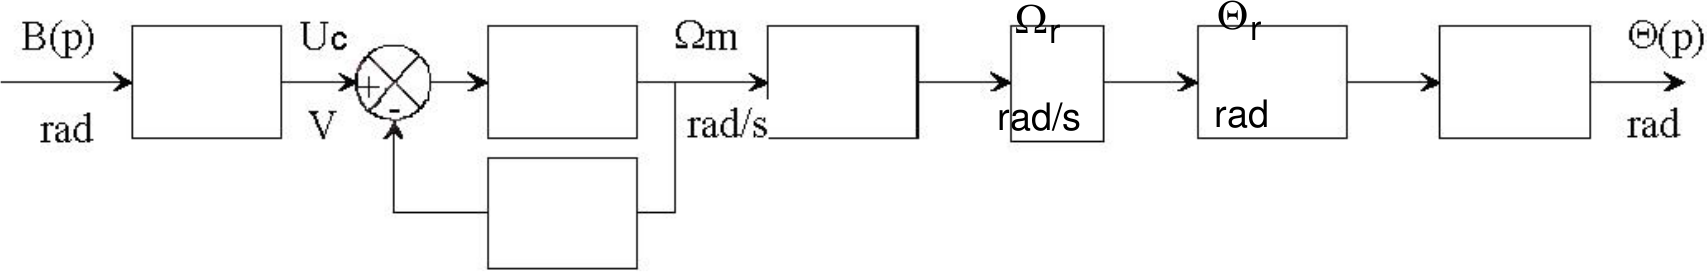
\includegraphics[width=.6\textwidth]{png/image4}
\end{center}

\item Refaire, sur votre copie, le diagramme fonctionnel de la chaîne d‘action
ci-dessus, mais cette fois-ci en précisant les fonctions de transfert de chaque\\
bloc.

Pour déterminer la fonction de transfert du moteur, $M(p)$, on dispose de sa
réponse indicielle (entrée unitaire) :

\begin{center}
 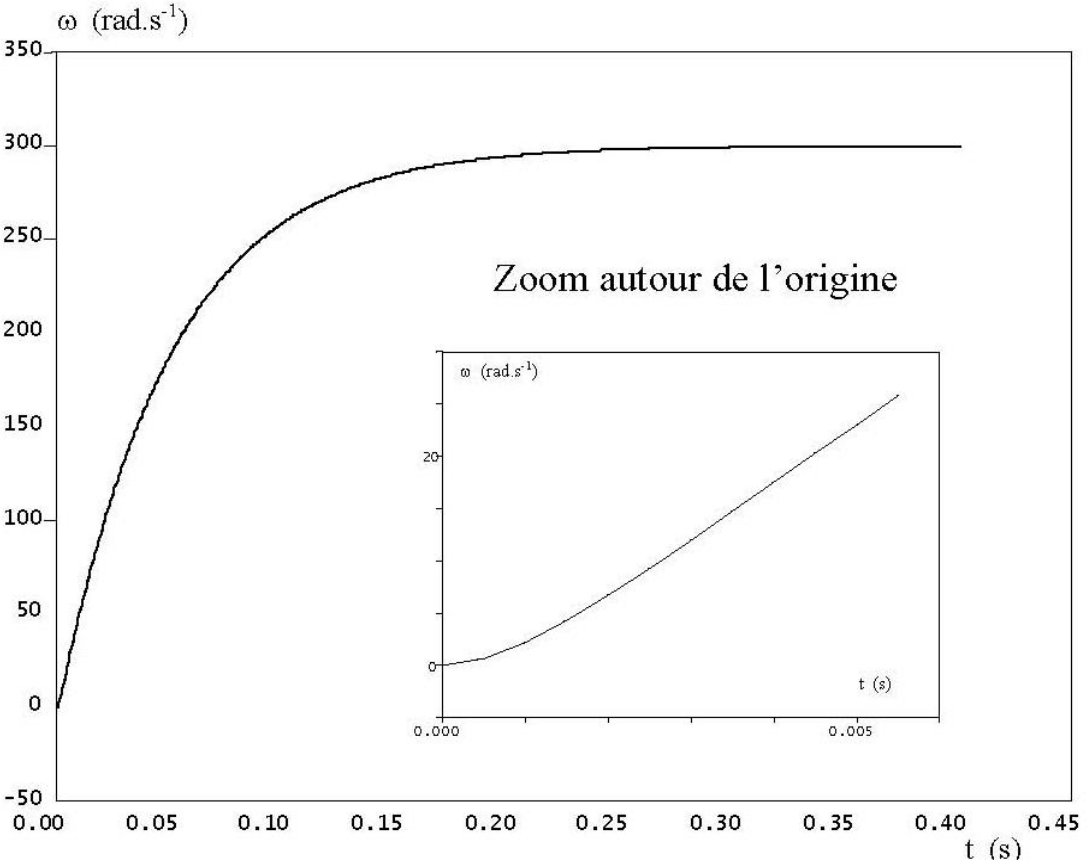
\includegraphics[width=.6\textwidth]{png/image5}
\end{center}


\item Quelle est la forme de la fonction de transfert du moteur et pourquoi ?

\item Quelle hypothèse pouvons-nous faire pour modéliser le système par un
système du 1\up{er}
ordre ?
NB : Pour démontrer ce raisonnement, déterminer la réponse temporelle d’un
système
du 2\up{ème} ordre apériodique, puis simplifier cette réponse avec votre
hypothèse et enfin
conclure.
Cette hypothèse vous semble-t-elle justifiée ici au vu de la réponse indicielle.


\item Identifier $M(p)$ à un 1\up{er} ordre. (Pour cela déterminer les
paramètres caractéristiques sur la courbe).


\item En déduire la fonction de transfert $M'(p)=\dfrac{\Omega_m(p)}{U_c(p)}$
du moteur équipé du retour                                                 
tachymétrique. Quels sont les avantages et les inconvénients de cette boucle de
retour ?\\

La fonction de transfert de la chaîne d‘action complète est donnée
approximativement par :
$H(p)=\dfrac{\Theta(p)}{B(p)}=K_c\dfrac{0,003}{\left(1+0,025p \right)p}$    
(Les angles d‘entrée et de sortie sont exprimés en radian).

Le véhicule est brusquement chargé à l‘arrière.


\item Tracer, SANS FAIRE DE CALCUL, l‘allure de la loi d‘entrée, puis l‘allure
de la réponse.
Justifier votre tracé. Est-ce satisfaisant ?\\


Pour remédier à ce problème on asservit le système en position en plaçant :
\begin{itemize}
 \item un capteur de position, de gain $K_{pos}$ , qui mesure l‘angle $\theta$,
\item un amplificateur de gain pur $A$.
\end{itemize}

\begin{center}
 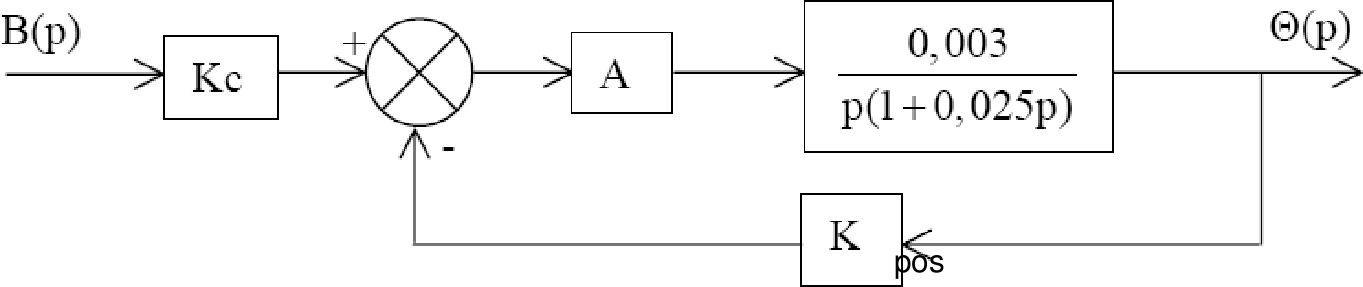
\includegraphics[width=.6\textwidth]{png/image6}
\end{center}


\item Déterminer la nouvelle fonction de transfert $\dfrac{\Theta(p)}{B(p)}$
ainsi que ses paramètres caractéristiques.


\item Expliquer en deux lignes pourquoi le problème a été remédié.

\item À partir de la courbe ci-contre, déterminer la quantité $AK_{pos}$ qui
permet d‘avoir le système le plus rapide. Calculer alors le temps de réponse à
5\% du système.

\begin{center}
 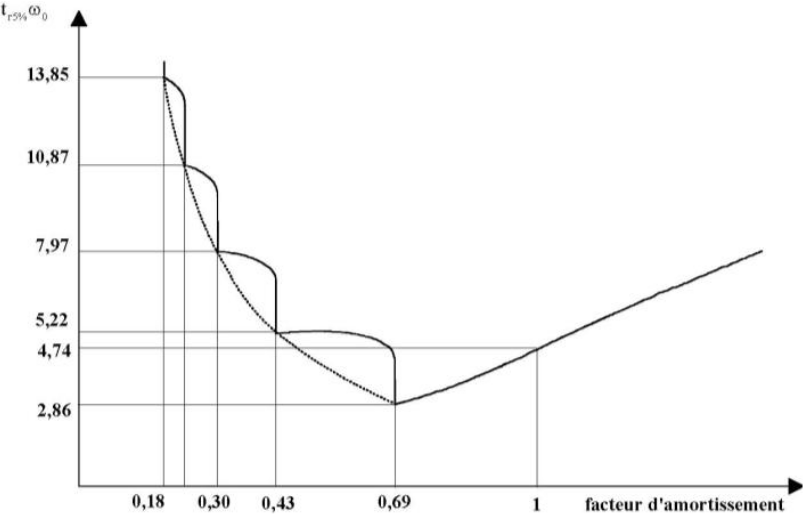
\includegraphics[width=.6\textwidth]{png/image7}
\end{center}
\end{enumerate}
\newpage

%--------------------------------------------

\exercice{Unité dentaire}
\textit{(Selon le concours E3A PSI 2007)}
\vspace{0.25cm}


\begin{minipage}[c]{.6\linewidth}
Le support de l'étude est une "unité dentaire" dont on donne un extrait du cahier des charges fonctionnel. Cet équipement a été conçu et réalisé dans le but d'une adaptabilité maximale aux différentes méthodes de travail des chirurgiens dentistes. Son ergonomie, sa maniabilité, son design, sa fiabilité en font une "unité universelle". Sa conception est modulaire avec une technologie avancée.

Le chirurgien dentiste possède une pédale et un pupitre de commande, qui lui permet de monter ou descendre verticalement le corps du patient, de l'incliner plus ou moins, et de positionner sa tête. Le patient pouvant prendre une position spatiale pertinente, tous les actes médicaux sont facilités.
\end{minipage}\hfill
\begin{minipage}[c]{.35\linewidth}
\begin{center}
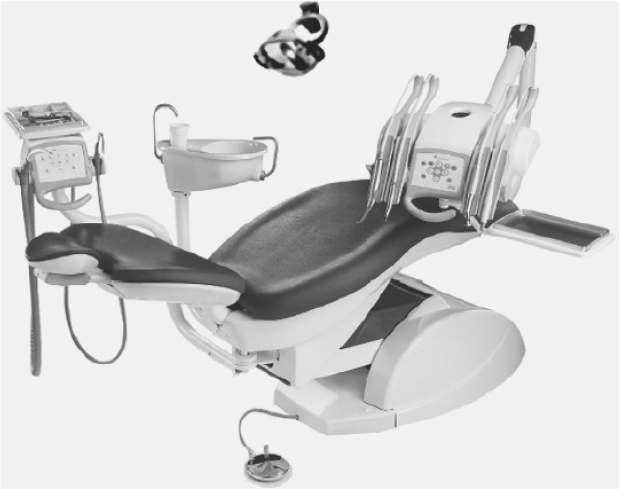
\includegraphics[width=.9\textwidth]{png/fig1-dentaire}
\end{center}
\end{minipage}

\begin{center}
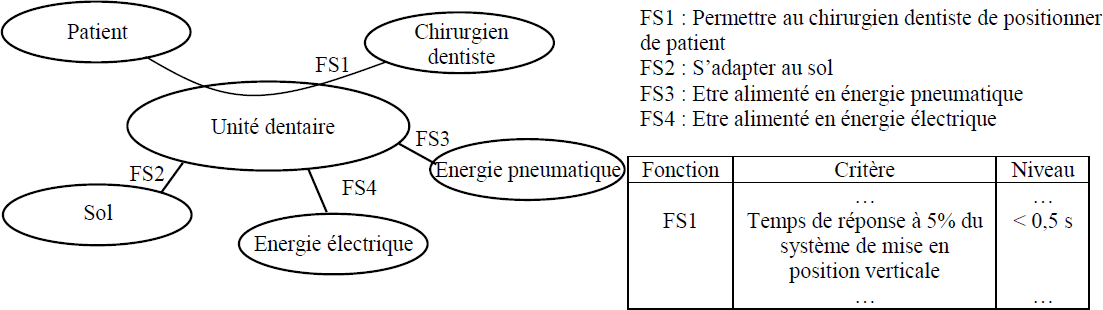
\includegraphics[width=.9\textwidth]{png/fig2-dentaire}
\end{center}

On s'intéresse dans ce sujet au critère de la FS1 concernant le temps de réponse du système permettant de mettre en position verticale le patient. 

Pour régler le patient en position verticale, le chirurgien dentiste appuie sur une pédale, plus ou moins fort. Un moteur électrique se met en route, sa vitesse de rotation dépend de l'appui plus ou moins profond du chirurgien dentiste sur la pédale. La vitesse de rotation du moteur est diminuée par un réducteur à engrenages. En sortie du réducteur à engrenages se trouve une vis dont la rotation $\Omega_v(p)$ entraîne, par un système vis-écrou, la translation du siège en hauteur. L'ensemble peut se représenter par le schéma bloc suivant. Le composant de fonction de transfert $C(p)$ est un correcteur :


\begin{center}
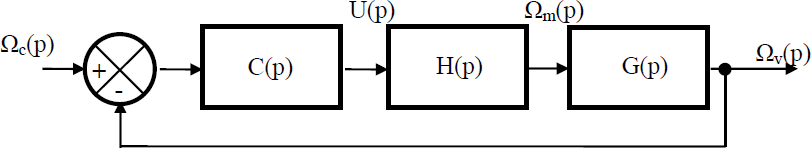
\includegraphics[width=.6\textwidth]{png/fig3-dentaire}
\end{center}

\subsubsection{Travail demandé}
\begin{enumerate}

\item Déterminer le nom des composants qui réalisent les fonctions $H(p)$ et $G(p)$.

\item Déterminer la fonction de transfert en boucle fermée du système $\dfrac{\Omega_v(p)}{\Omega_c(p)}$.\\

Les équations du moteur utilisé sont les suivantes :
$$
u(t)=e(t)+Ri(t)+L\dfrac{di(t)}{dt} \quad e(t) = k_e \omega_m(t) \quad J\cdot\dfrac{d\omega_m(t)}{dt} = C_m(t)-f\omega_m(t) \quad C_m(t)=k_m \cdot i(t)
$$

On note $u(t)$ tension du moteur, $e(t)$, la force contre électro motrice du moteur, $i(t)$ l'intensité dans le moteur, $C_m(t)$ le couple exercé par le moteur et $\omega_m(t)$ la vitesse angulaire du moteur. Les grandeurs physiques $R$, $L$, $k_e$, $J$, $f$ et $k_m$ sont des constantes.

\item En supposant les conditions initiales nulles, exprimer ces équations dans le domaine de Laplace.

\item Montrer que, dans le domaine de Laplace, la relation entre $\Omega_m(p)$ et $U(p)$ peut s'écrire sous la forme d'une fonction de transfert du second ordre. On déterminera les différentes constantes.\\

Si on utilise un correcteur proportionnel, l'application numérique des grandeurs physiques permet de trouver la fonction suivante : $\dfrac{\Omega_v(p)}{\Omega_c(p)} =\dfrac{K_T}{1+T_T p}$ avec $K_T=0,9$ et $T_T=0,1 s.$.

\item Déterminer $\omega_v(t)$ lorsque le chirurgien dentiste demande un échelon de rotation $\omega_c(t)=\omega_{c0}\cdot u(t)$. Exprimer le résultat en fonction de $\omega_{C0}$, $K_T$ et $T_T$.

\item Déterminer le temps de réponse à 5\% du système et effectuer l'application numérique. Conclure vis-à-vis du cahier des charges.\\

Le patient, initialement immobile, bouge verticalement selon le déplacement $x_v(t)$ tel que $\dfrac{dx_v(t)}{dt} = a\omega_v(t)$ avec $a$ constante qui représente le pas réduit de la vis. 

\item Déterminer la transformée de Laplace $X_v(p)$ de $x_v(t)$.

\item Déterminer $x_v(t)$ en fonction de $a$, $K_T$, $T_T$ et $\omega_{c0}$.\\


Si on utilise un correcteur proportionnel, dérivé et intégral, l'application numérique des grandeurs physiques permet de trouver la fonction suivante : $\dfrac{\Omega_v(p)}{\Omega_c(p)} = \dfrac{1}{1+2p+p^2}
$

\item Déterminer $\omega_v(t)$ lorsque le chirurgien dentiste demande un échelon de rotation $\omega_c(t)=\omega_{c0}\cdot u(t)$.

\item Déterminer si le temps de réponse à 5\% est plus faible  ou plus grand que dans le cas précédent. Conclure vis-à-vis du cahier des charges.
\end{enumerate}
\newpage

%----------------------------------------------------------------------------------------
%	Études féquentielles
%----------------------------------------------------------------------------------------
\section{Études fréquentielles}

%--------------------------------------------

\exercice{Tracé \& interprétation d'un diagramme de Bode}
On se propose de d\'eterminer le comportement fr\'equentiel d'un syst\`eme dont la fonction de transfert est donn\'ee :
\begin{description}
\item \[H(p)=\frac{10}{(1+0,003.p+0,25.p^2).(1+0,1.p)}\]
\end{description}
\begin{enumerate}
\item Proposer une m\'ethode pour tracer le diagramme de Bode, en gain et phase, de la fonction de transfert $H(p)$.
\item \'Ecrire les fonctions de transfert isochrones de $H_1(p)$ et $H_2(p)$.
\item Tracer les diagrammes asymptotiques, puis r\'eels, de chacune des fonctions $H_1(j\omega)$ et $H_2(j\omega)$.
\item En d\'eduire le diagramme asymptotique puis réel de $H(j\omega)$.
\item On sollicite le syst\`eme avec les entr\'ees sinuso\"idales :
\begin{itemize}
\item $e_1(t)=3.\sin(1,2.t)$
\item $e_2(t)=3.\sin(120.t)$
\end{itemize}
Donner pour chacune des entr\'ees la r\'eponse en r\'egime permanent.
\end{enumerate}

\correction{ % Answer
\begin{enumerate}
\item On pose $H(p)=H_1(p)H_2(p)$ tel que $H_1(p)$ et $H_2(p)$ soient des fonctions de transfert élémentaires du première ordre ou du deuxième ordre.
\item \[H_1(p)=\frac{1}{1+0,003p+0,25p^2} \mbox{ et } H_2(p)=\frac{10}{1+0,1p}\]\\
\textit{Remarque : On obtient les fonctions de transfert isochrones en remplaçant $p$ par $j\omega$ pour ensuite faire une étude fréquentielle du système.}
\item \underline{Tracés assymptotiques :}\\
Cf. Cours\\
\underline{Tracés réels :}
\begin{itemize}
\item Étude de $H_1(j\omega)$\\
\[\frac{1}{\omega_0^2}=0,25 \mbox{ d'où } \omega_0=0,5 s^{-1}\]
\[\frac{2\xi}{\omega_0}=0,03 \mbox{ d'où } \xi=0,03\frac{\omega_0}{2}=0,0125<0,7\]
Il y a donc résonnance à $\omega_r=\omega_0\sqrt{1-\xi^2}=0,5 s^{-1}$ avec un coefficient de surtension : \( Q_{dB}=-20\log(2\xi \sqrt{1-\xi^2})=32 dB \)
\end{itemize}
Cf. Cours
\item En sommant les deux diagrammes de Bode réels déterminés précédemment, on obtient celui de $H(j\omega)$.\\
Cf. Cours pour le tracé
\item Cf. Définition d'une étude fréquentielle à l'aide des diagrammes de Bode.
\end{enumerate}
}
\newpage

%--------------------------------------------

\exercice{Études fréquentielles à l'aide du diagramme de Bode}
On se propose de déterminer le comportement fréquentiel des systèmes dont leur fonction de transfert est donnée :
\begin{equation}
H_1(p)=K\frac{1+\tau_1 p}{1+\tau_2 p}
\end{equation}
avec $\tau_1=0,9s$, $\tau_2=0,1s$ et $K=8$

\begin{equation}
H_2(p)=\frac{25}{p(1+0,5p+0,25p^2)}
\end{equation}

\subsubsection{Travail demandé}
\begin{enumerate}
\item Tracer le diagramme de Bode assymptotique, puis réel, des deux systèmes.
\item Déterminer les coordonnées de l'extremum en phase du système défini par $H_1(p)$.
\end{enumerate}

\correction{
\begin{enumerate}
\item Diagramme de Bode de $H_1(p)$ :
\begin{center}
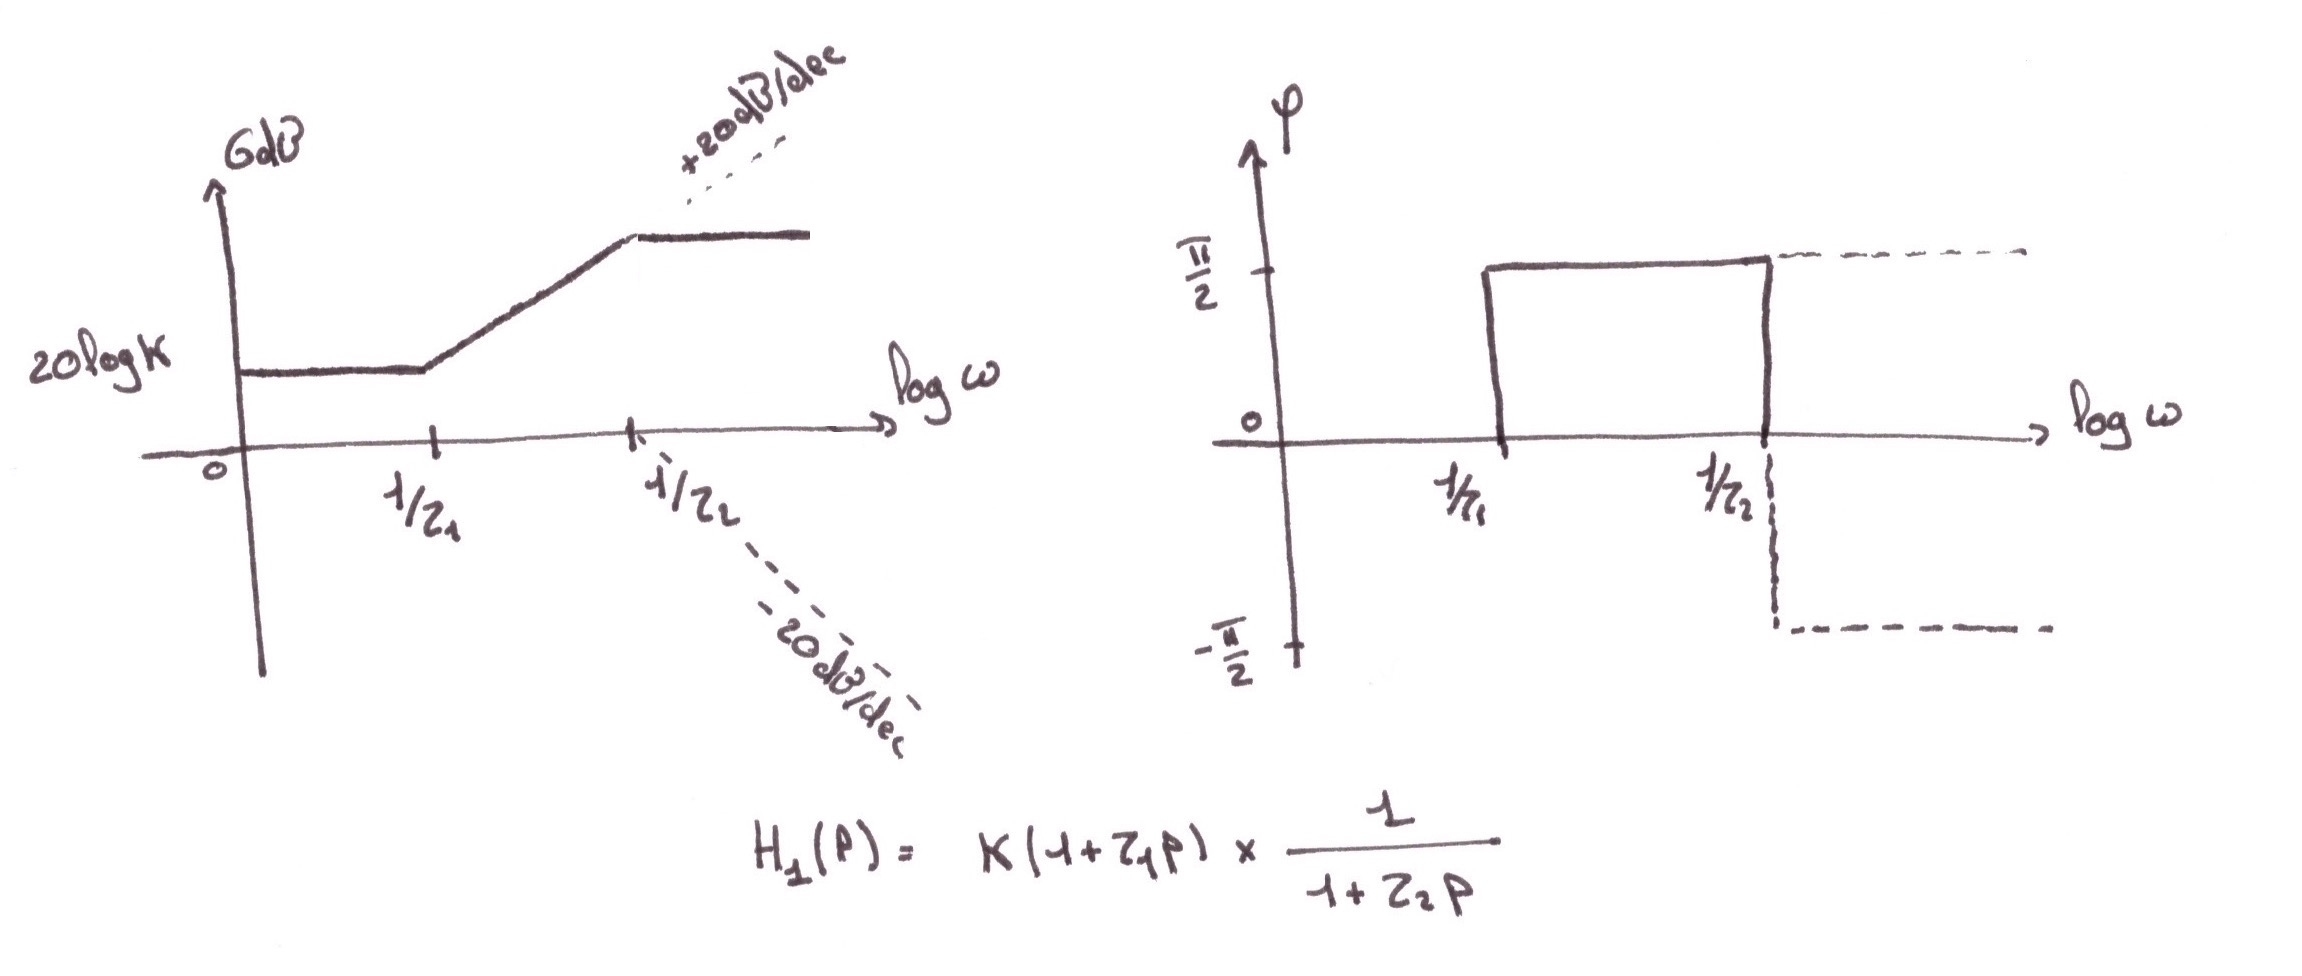
\includegraphics[width=0.5\paperwidth]{png/H1.jpeg}
\end{center}
Diagramme de Bode de $H_2(p)$ :
\begin{center}
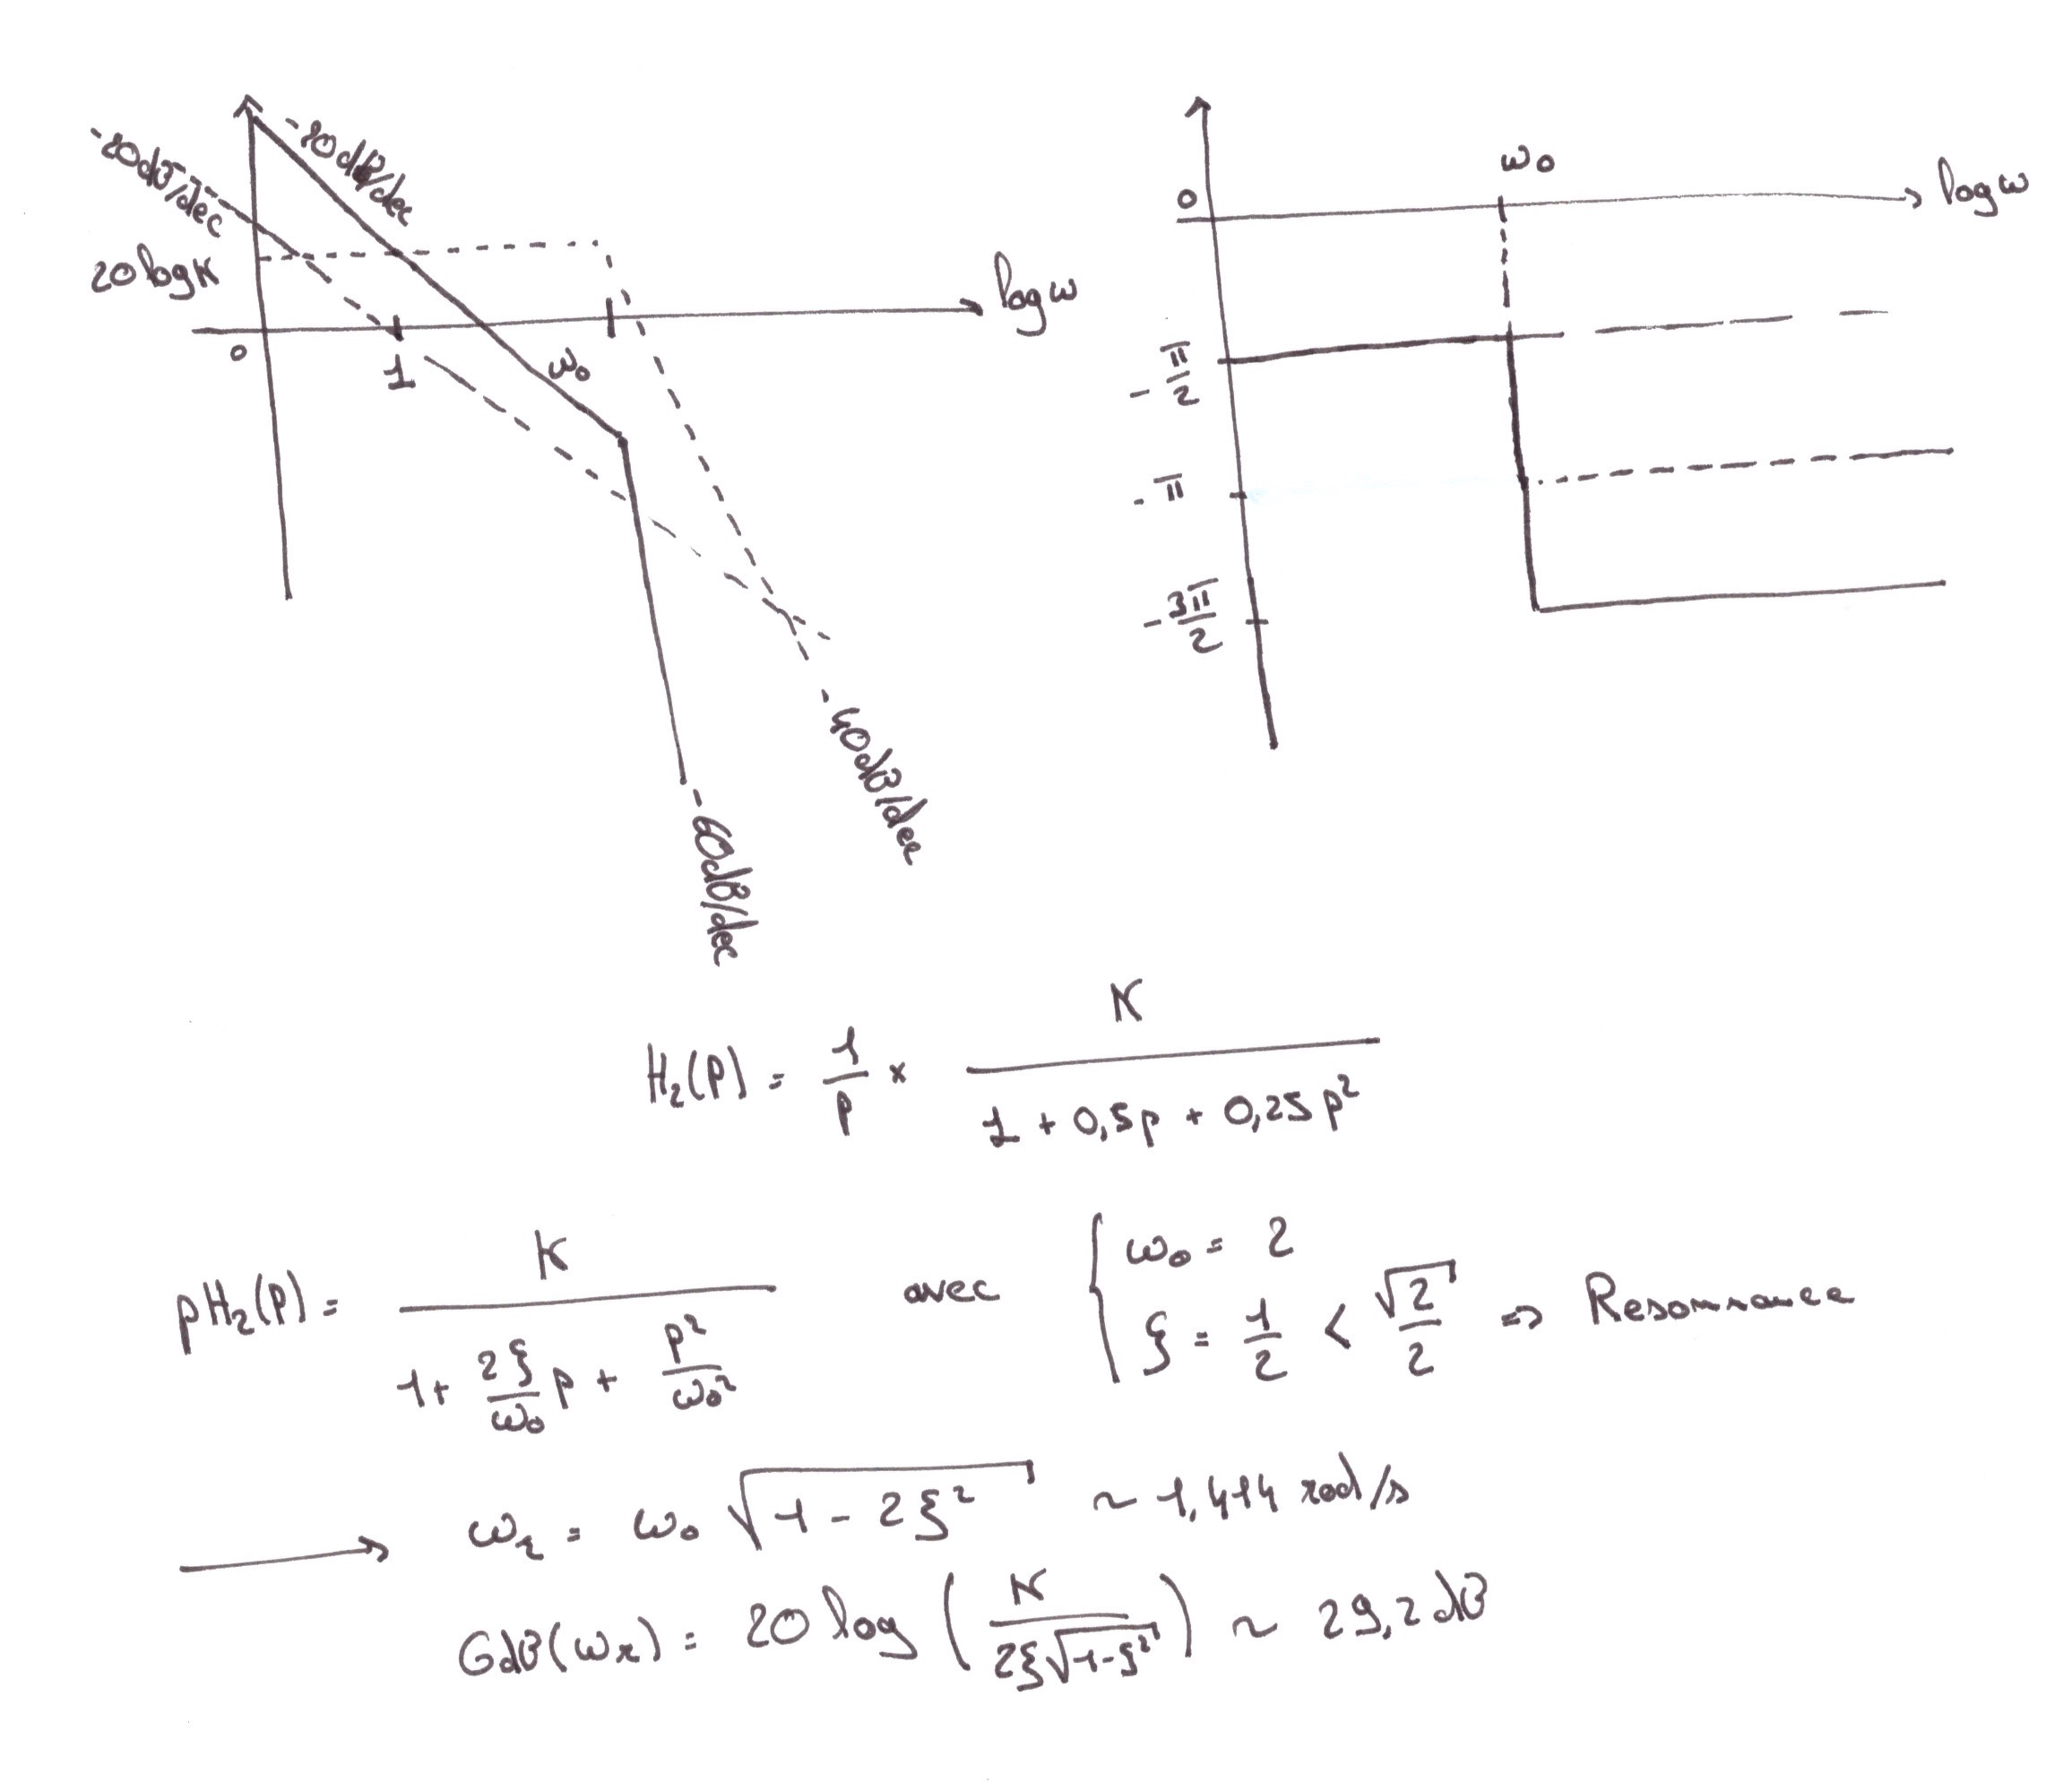
\includegraphics[width=0.5\paperwidth]{png/H2.jpeg}
\end{center}
\item \[ \phi=arg(H_1(j\omega))=arctan(\tau_1 \omega)-arctan(\tau_2 \omega) \] \\
RAPPEL : $arctan'(\theta)=\frac{1}{1+\theta^{2}}$\\
\[ \frac{d \phi}{d \omega}= \frac{\tau_1}{1+(\tau_1 \omega)^{2}}-\frac{\tau_2}{1+(\tau_2 \omega)^{2}}=0 \]
\[ \omega=\sqrt{\frac{1}{\tau_1 \tau_2}}=3,333rad/s \]
d'où $\phi=53^{\circ} $
\end{enumerate}
}
\newpage

%--------------------------------------------

\exercice{Réponse fréquentielle}
On excite un système linéaire du second ordre par un signal sinusoïdal $e(t)=e_0.\sin(\omega t)$ de fréquence $f=\frac{\omega}{2.\pi}$ variable de $0$ à $500Hz$. Pour $e_0=50mV$, on obtient la sortie $s(t)=s_0.sin(\omega t +\Phi)$ dont l'amplitude $s_0$ est donnée en fonction de la fréquence sur la courbe ci-dessous.

\begin{center}
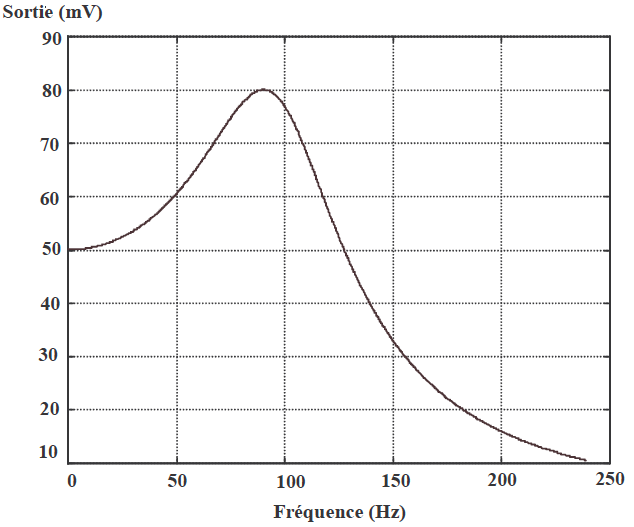
\includegraphics[scale=0.5]{png/graphe2nd.png}
\end{center}

\subsubsection{Travail demandé}
\begin{enumerate}
\item Écrire la fonction de transfert du système et exprimer son module et son argument.
\item Donner les expressions des variables suivantes et utiliser la figure pour calculer leur valeur :
\begin{itemize}
\item le gain statique.
\item la pulsation de résonnance $\omega_R$.
\item le facteur d'amortissement $\xi$.
\item la pulsation propre $f_0$ du système non amortie (pulsation naturelle).
\item la fréquence $f_{C-6dB}$ de coupure à $6dB$.
\end{itemize}
\end{enumerate}

\correction{
\begin{enumerate}
\item \[ H(j\omega)=\frac{K}{1+j2\xi\frac{\omega}{\omega_0}-(\frac{\omega}{\omega_0})^2} \]
Module : \(|H(j\omega)|=\frac{|K|}{\sqrt{(1-(\frac{\omega}{\omega_0})^2)^2+(2\xi \frac{\omega}{\omega_0})^2}} \)\\
Argument : \( arg(H(j\omega))=-\arctan(\frac{2\xi \frac{\omega}{\omega_0}}{1-(\frac{\omega}{\omega_0})^2}) \)\\
\textit{Remarque : $s(t)=|H(j\omega)|e_0 \sin(\omega.t+arg(H(j\omega))$}
\item Expressions :
\begin{itemize}
\item le gain statique : $|H(j\omega=0)|=\frac{|S(j\omega=0)|}{|E(j\omega=0)|}=|K|$ avec  $|S(j\omega=0)|$ l'amplitude de $s(t)$ à la pulsaton nulle et $|E(j\omega=0)|=e_0$ l'amplitude de $e(t)$ à la pulsation nulle. D'où :
\[|K|=\frac{|S(j\omega=0)|}{e_0}=1\]
\item le facteur d'amortissement $\xi<\frac{\sqrt{2}}{2}$ (car résonance).
\item le facteur de surtension $|S(j\omega_r)|=\frac{|K.e_0|}{2\xi \sqrt{1-\xi^2}}$. D'où :
\[ 4\xi^4-4\xi^2+(\frac{|K.e_0|}{|S(j\omega_r)|})^2=0\]
En posant $X=\xi^2$ et en sachant que $0<\xi<\frac{\sqrt{2}}{2}$ : $\xi=0,33$.
\item la pulsation de résonnance : $\omega_r=\omega_0\sqrt{1-2\xi^2}$
\item la pulsation propre $f_0=\frac{\omega_0}{2 \pi}$\\
On en déduit : $f_0=\frac{\omega_0}{2\pi}=\frac{f_r}{\sqrt{1-2\xi^2}}=101,9Hz$.
\item $|S(j\omega_{C-6dB})|=|H(j\omega_{C-6dB})|e_0=10^{\log(|K|)-\frac{6}{20}}e_0=25mV$\\
On en déduit à partir du graphique $f_{C-6dB}=170Hz$.
\end{itemize}
\end{enumerate}
}
\newpage

%----------------------------------------------------------------------------------------
%	PROBLEMES
%----------------------------------------------------------------------------------------
\section{Problèmes}

%--------------------------------------------

\probleme{Mod\'elisation d'une servo-valve}

\subsubsection{I. Pr\'esentation}
On s'int\'eresse ici \`a la loi de comportement d'un v\'erin hydraulique d\'epla\c{c}ant un chariot.
Le syst\`eme se compose de :

\begin{itemize}
\item Un moteur hydraulique lin\'eaire (v\'erin) qui transforme l'\'energie hydraulique en \'energie m\'ecanique. Il est
form\'e de deux chambres 1 et 2, s\'epar\'ees par un piston, de section S, perc\'e d'un trou de fuite de section
tr\`es faible par rapport \`a $S$.
\item Le piston est solidaire d'un chariot, de masse M, dont le d\'eplacement est rep\'er\'e par $x(t)$. Le frottement entre
le chariot et le b\^ati est visqueux (coefficient $\mu$).
\item La circulation du fluide, suppos\'e incompressible, est assur\'ee par une servo-valve dont le d\'ebit volumique
q est proportionnel au courant de r\'eglage $i(t)$ 
\end{itemize}
On note $P_i$ la pression dans la chambre $i$ \`a l'instant $t$. Le d\'ebit de fuite $q_f$ entre les chambres 1 et 2 est
suppos\'e ob\'eir \`a la loi des \'ecoulements laminaires: $q_f(t) = R (p_1(t) - p_2(t))$. On appelle $F(t)$ la force exerc\'ee par l'huile sur
le piston.\\
\hspace*{0mm}
\begin{center}
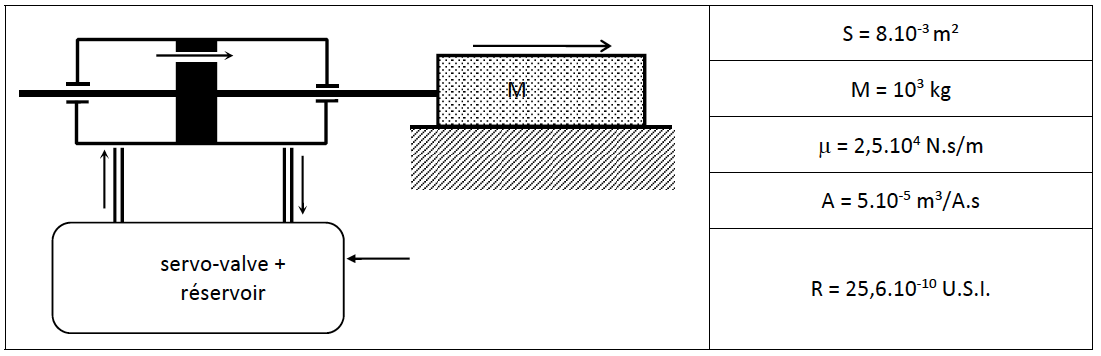
\includegraphics[scale=0.4]{png/img1_prob1.png}
\end{center}
\hspace*{0mm}
Les \'equations d\'ecrivant le comportement des diff\'erents \'el\'ements sont :
\begin{itemize}
\item Comportement de la servo-valve : $ q(t)=A.i(t)$
\item Relation reliant le d\'eplacement du piston aux diff\'erents d\'ebits : $q(t)=q_f(t)+S.\frac{dx(t)}{dt}$
\item Relation liant l'effort de l'huile sur le piston en fonction du d\'ebit de fuite : $F(t)=\frac{S}{R}.q_f(t)$
\item Principe fondamental de la dynamique appliqu\'e au chariot : $M.\frac{d^2x(t)}{dt^2} = F(t)-\mu.\frac{dx(t)}{dt}$
\end{itemize}
\newpage

\subsubsection{II. Travail demand\'e}
\begin{enumerate}
\item D\'efinir l'entr\'ee et la sortie de ce syst\`eme
\item Ecrire les \'equations de comportement dans le domaine de Laplace (on se placera dans les
conditions de Heaviside)
\item Pr\'eciser sur le sch\'ema bloc ci-dessous le nom des grandeurs physiques ainsi que les
fonctions de transfert\\
\hspace*{0mm}
\begin{center} 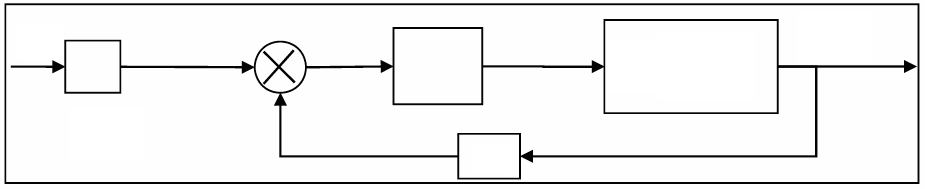
\includegraphics[scale=0.45]{png/img2_prob1.png}\end{center}
\hspace*{0mm}
\item D\'eterminez la fonction de transfert de ce syst\`eme H(p). Pr\'eciser l'ordre de celle-ci.
\item Donner les grandeurs caract\'eristiques de celle-ci en pr\'ecisant les unit\'es.
\item On soumet le syst\`eme \`a un \'echelon d'intensit\'e $I_0$. Pr\'ecisez la fonction de Laplace
correspondante.
\item Donner la relation entre la position et la vitesse puis calculer la vitesse du chariot en r\'egime
permanent.
\item Tracer l'allure de la vitesse.
\item D\'eterminer la r\'eponse $x(t)$ en fonction de $K$, $I_0$ et $\tau$. (on pourra judicieusement s'appuyer
sur l'expression de $v(t)$)
\item On soumet maintenant le syst\`eme \`a une entr\'ee sinuso\"{i}dale d'intensit\'e $I_0$ et de pulsation $\omega_0=\frac{1}{\tau}$. Pr\'ecisez la fonction de Laplace correspondante.
\item D\'eterminer l'expression de $x(t)$ en r\'egime permanent en fonction de $K$, $I_0$ et $\tau$.
\end{enumerate}

\correction{ % Answer
\begin{enumerate}
\item Entrée : courant de réglage de la servo-valve, $i(t)$\\
Sortie : déplacement de la masse $M$, $x(t)$
\item $Q(p)=AI(p)$\\$Q(p)=Q_f(p)+SpX(p)$\\$F(p)=\frac{S}{R}Q_f(p)$\\$Mp^2X(p)=F(p)-\mu p X(p)$
\item Schéma bloc :
\begin{center}
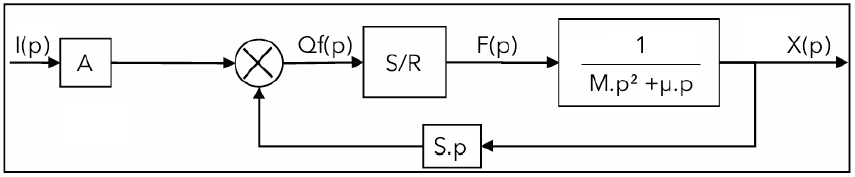
\includegraphics[scale=0.4]{png/img2_prob1-cor.png}
\end{center}
\item Schéma bloc :
\begin{center}
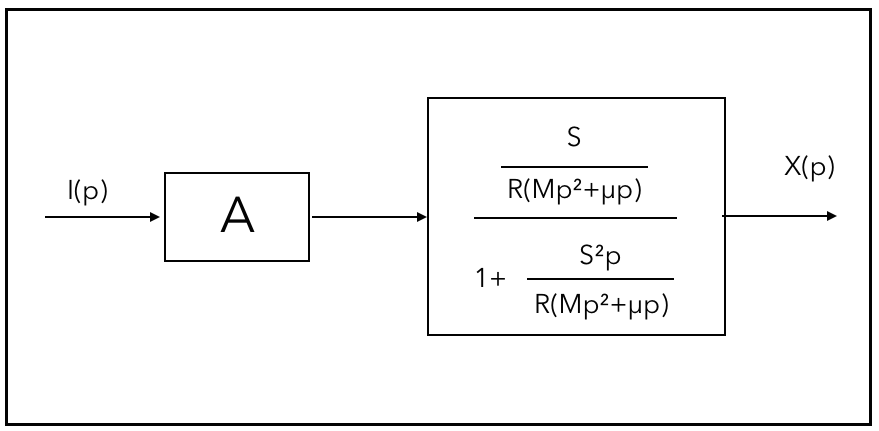
\includegraphics[scale=0.25]{png/img2_prob1-cor2.png}
\end{center}
\[ H(p)=\frac{X(p)}{I(p)}=\frac{\frac{AS}{S^2+R\mu}}{p(1+\frac{RM}{S^2+R\mu}p)} \]
Il s'agit d'une fonction de transfert d'un système du deuxième ordre (première ordre multiplié par un intégrateur pur)
\item On pose \( H(p)=\frac{1}{p}\frac{K}{1+\tau p} \) avec \( K=\frac{AS}{S^2+R\mu} \) (en $m.A^{-1}.s^{-1}$) et \( \tau=\frac{RM}{S^2+R\mu} \) (en $s^{-1}$)\\
\textit{Remarque : l'unité $s^{-1}$ de $K$ vient de l'intégrateur pur}
\item \( I(p)=\frac{I_0}{p} \)
\item Comme \( v(t)=\frac{dx(t)}{dt} \), \( V(p)=pX(p) \)
\[ \lim_{p \rightarrow +\infty} v(t)=\lim_{p \rightarrow 0} pV(p) = \lim_{p \rightarrow 0} p^2X(p)=\lim_{p \rightarrow 0} pH(p)I_0=\lim_{p \rightarrow 0} \frac{KI_O}{1+\tau p}=KI_0 \]
\item Allure de la vitesse $V(t)$ :
\begin{center}
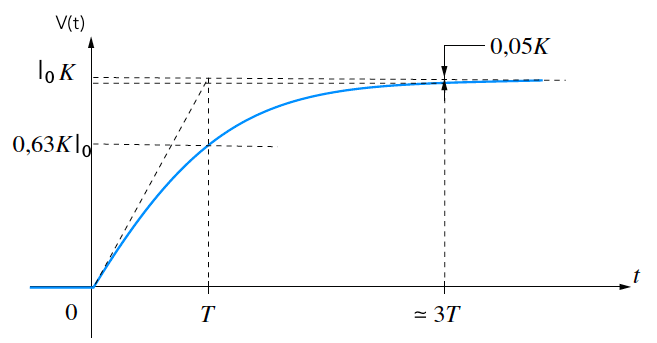
\includegraphics[scale=0.5]{png/courbe-prob1-cor.png}
\end{center}
\item \( v(t)=KI_0(1-e{-\frac{t}{\tau}}) \) car premier ordre\\
\( x(t)=\int_0^t v(t)dt=\int_0^t KI_0(1-e^{-\frac{t}{\tau}})dt=KI_0[t+\tau e^{-\frac{t}{\tau}}-\tau] \)
\item \textit{RAPPEL : $\sin(\omega t)\mathcal{U}(t) \rightarrow \frac{\omega}{p^2+\omega^2}$ et $\cos(\omega t)\mathcal{U}(t) \rightarrow \frac{p}{p^2+\omega^2}$}\\
\( i(t)=I_0\sin(\omega_0 t) \rightarrow I(p)=\frac{I_0\omega_0}{p^2+\omega_0^2}=\frac{\frac{I_0}{\tau}}{p^2+\frac{1}{\tau^2}} \) où $\omega_0=\frac{1}{\tau}$
\item \[ X(p)=\frac{1}{p}\frac{K}{1+\tau p}\frac{I_0\frac{1}{\tau}}{p^2+\frac{1}{\tau^2}}=\frac{KI_0 \tau}{p}-\frac{\frac{KI_0 \tau}{2}}{\frac{1}{\tau}+p}-\frac{\frac{KI_0 \tau}{2}(p+\frac{1}{\tau})}{p^2+\frac{1}{\tau^2}} \]
\[ x(t)=\frac{KI_0 \tau}{2}(2-\cos(\frac{t}{\tau})-\sin(\frac{t}{\tau})-e^{-\frac{t}{\tau}}) \]
En régime permanent : \( x(t)=\frac{KI_0 \tau}{2}(2-\cos(\frac{t}{\tau})-\sin(\frac{t}{\tau})) \)
\end{enumerate}
}
\newpage

%--------------------------------------------

\probleme{Cam\'era de poursuite (SPEEDCAM)}

\subsubsection{I. Pr\'esentation}
L'\'etude porte sur la cam\'era de poursuite SPEDDCAM utilis\'ee dans de nombreux championnats pour filmer les performances des sportifs. La cam\'era est fix\'ee sur un chariot se d\'epla\c{c}ant sur un rail.
\\ \hspace*{0mm}
\begin{center}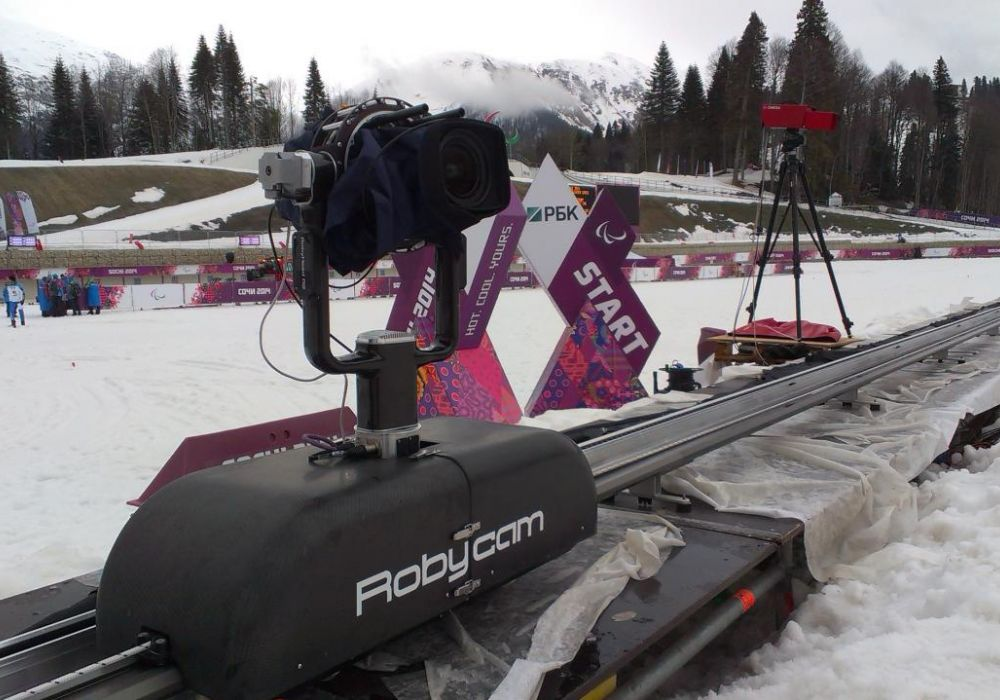
\includegraphics[scale=0.22]{png/img1_prob2.jpg} 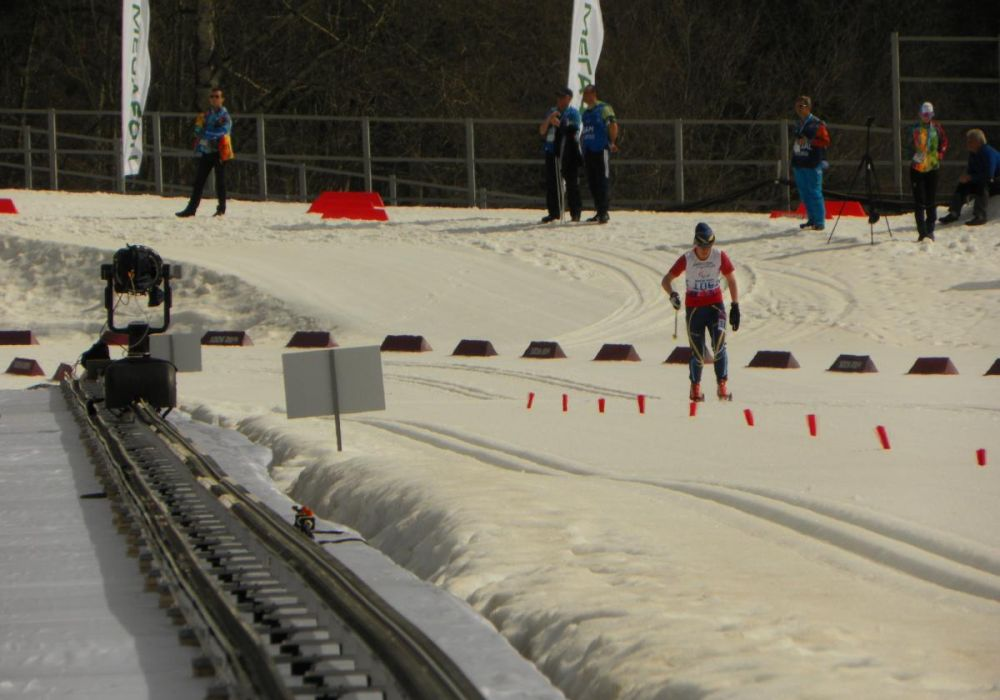
\includegraphics[scale=0.22]{png/img2_prob2.jpg}\end{center}
\hspace*{0mm}
\\Un capteur optique permet de mesurer la position de la cam\'era par rapport au comp\'etiteur. Un calculateur d\'etermine la consigne n\'ecessaire pour suivre le comp\'etiteur, transmise sous forme de tension de commande \`a l'asservissement du chariot. Le chariot est asservi en vitesse comme le montre le sch\'ema fonctionnel suivant :
\\ \hspace*{0mm}
\begin{center}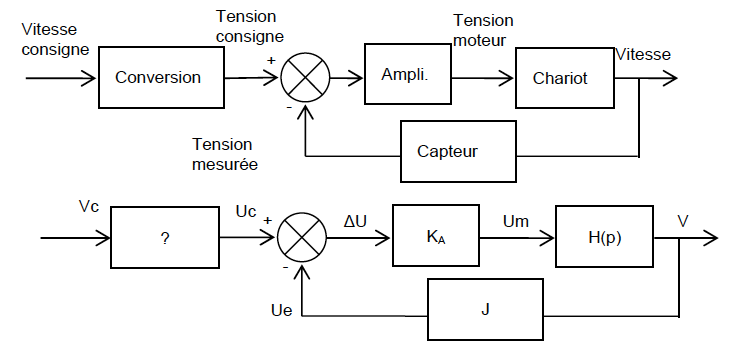
\includegraphics[scale=0.6]{png/bloc1_prob2.png}\end{center}
\hspace*{0mm}
\\ Le chariot est actionn\'e par un moteur \'electrique pilot\'e par sa tension d'entr\'ee $u_m(t)$. Cette tension est obtenue \`a l'aide d'un amplificateur fournissant une tension $u_m(t)$ proportionnelle \`a la tension de commande $\Delta U$ (gain $K_A = 500$). Un capteur de vitesse mesure la vitesse $v(t)$ et renvoit une information de tension $u_e(t)$
proportionnelle \`a la vitesse $v$ (gain $J = 0,3 V.s/m$).


\begin{enumerate}
\item D\'eterminer la fonction \`a mettre dans le convertisseur ("$?$") pour que $V$ soit asservie sur
$Vc$ (donc pour que $V$ soit compar\'ee \`a $Vc$).
\end{enumerate}

\subsubsection{II. Mod\'elisation du comportement du chariot}
Le chariot \'etant relativement complexe, il est impossible de donner a priori un mod\`ele de comportement $H(p)$ comme pour le capteur de vitesse ou l'amplificateur. Afin de mod\'eliser son comportement, on choisit de faire une mesure et de proposer un mod\`ele simple repr\'esentatif. La courbe (cf. graphe suivant) montre la r\'eponse obtenue par le capteur de vitesse lorsqu'un \'echelon de tension $u_m(t) = u_0.u(t)$ (avec $u_0 = 70 V$) est appliqu\'e en entr\'ee. ($u(t)$ : fonction de heaviside).
\\ On choisit un mod\`ele simple du premier ordre pour identifier le comportement du chariot, soit : \(H(p)=\frac{K_c}{1+\tau .p}\) o\`u $K_c$ et $\tau$ sont \`a d\'eterminer \`a l'aide de la courbe.

\begin{enumerate}
\item Exprimer $U_e(p)$ en fonction de $U_m(p)$.
\item D\'eterminer $K_c$ \`a l'aide de la courbe. Quelle est son unit\'e ?
\item D\'eterminer $\tau$ \`a l'aide la courbe par trois m\'ethodes. A partir des trois valeurs obtenues,
proposer une valeur de $\tau$ pertinente.\\
\hspace*{0mm}
\begin{center} 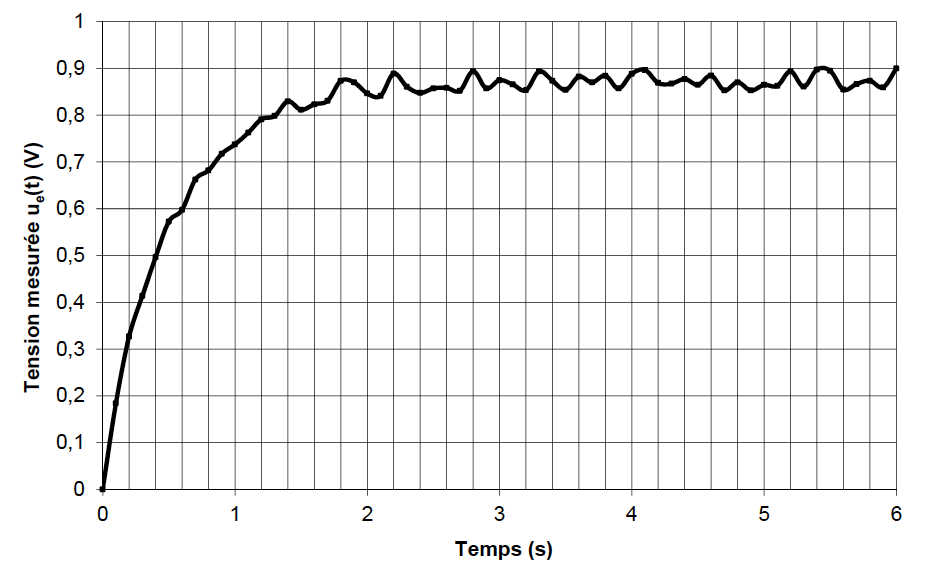
\includegraphics[scale=0.45]{png/courbe_prob2.png}\end{center}
\hspace*{0mm}
\end{enumerate}
\newpage

\subsubsection{III. Etude des performances du syst\`eme en boucle ferm\'ee}
On cherche maintenant \`a caract\'eriser les performances du syst\`eme asservi, c'est \`a dire la stabilit\'e, la rapidit\'e et la pr\'ecision.

\begin{enumerate}
\item Calculer la fonction de transfert \(H_T(p) = \frac{V(p)}{V_c(p)}\) du chariot asservi. D\'eterminer les caract\'eristiques de cette fonction de transfert.

\item En calculant la valeur \`a convergence de $v(t)$ suite \`a une entr\'ee en \'echelon $v_c(t)=V_{c0}.u(t)$. D\'eterminer si le syst\`eme est pr\'ecis. Comment augmenter cette pr\'ecision ?

\item D\'eterminer la rapidit\'e du syst\`eme. Comment augmenter la rapidit\'e ? Quelle sera la cons\'equence sur la pr\'ecision ?
\end{enumerate}

\subsubsection{IV. Am\'elioration de la pr\'ecision}
Une m\'ethode classique pour augmenter la pr\'ecision est d'ajouter un int\'egrateur $\frac{1}{p}$ dans la cha\^ine directe (voir figure ci dessous). Cet ajout est facile en amont de l'amplificateur. On d\'esigne par " correcteur " cet \'el\'ement rajout\'e, destin\'e \`a am\'eliorer le comportement de l'asservissement.
\\ \hspace*{0mm}
\begin{center} \includegraphics[scale=0.5]{png/bloc2_prob2.png}\end{center}
\hspace*{0mm}

\begin{enumerate}
\item Calculer la fonction de transfert \(H_{cor}(p)=\frac{V(p)}{V_c(p)}\) du chariot asservi. Pr\'eciser l'ordre de la fonction obtenue.
\item D\'eterminer si le syst\`eme est pr\'ecis.
\end{enumerate}

\correction{ % Answer
\textbf{Partie I}
\begin{enumerate}
\item La fonction du convertisseur est un gain $J$ qui convertit une vitesse en tension.
\end{enumerate}

\textbf{Partie II}
\begin{enumerate}
\item \( U_e(p)=H(p).J.U_m(p) \)
\item Lecture graphique de la coube $U_e(t)$ :
\begin{center}
\includegraphics[scale=0.5]{png/courbe-prob2-cor.png}
\end{center}
\item \( \tau=0,5s \)
\end{enumerate}

\textbf{Partie III}
\begin{enumerate}
\item \( H_T(p)=\frac{V(p)}{V_c(p)}=\frac{JK_AH(p)}{1+JK_AH(p)}=\frac{\frac{K_cK_AJ}{1+JK_AK_c}}{1+\frac{\tau}{1+JK_AK_c}p} \)\\
\(H_T(p)=\frac{K_T}{1+\tau_Tp} \) avec \( K_T=\frac{K_cK_AJ}{1+JK_AK_c} \) et \( \tau_T=\frac{\tau}{1+JK_AK_c} \)
\item \( v_c(t)=v_{c0}\mathcal{U(t)} \rightarrow V_c(p)=\frac{V_{c0}}{p} \)\\
\( \lim_{t \to +\infty}v(t)=\lim_{p \to 0}pV(p)=\lim_{p \to 0}\frac{K_T}{1+\tau_T p}V_{c0}=K_TV_{c0} \)\\
Le système est précis seulement si $v(t) \rightarrow_{t \to +\infty} V_{c0}$ donc $K_T$ doit tendre vers $1$. Comme $K_T=\frac{K_cK_AJ}{1+JK_AK_c}$ il faut pouvoir augmenter $K_A$, en pratique $K_A \rightarrow +\infty$ est impossible.
\item Pour un premier ordre, $t_{5\%} \simeq 3\tau_T = \frac{3\tau}{1+JK_AK_c}$\\
Pour augmenter la rapidité, il faut augmenter $K_A$.
\end{enumerate}

\textbf{Partie IV}
\begin{enumerate}
\item \( H_{cor}(p)=\frac{V(p)}{V_c(p)}=J\frac{H(p)\frac{K_A}{p}}{1+H(p)J\frac{K_A}{p}}=\frac{1}{1+\frac{1}{JK_AK_c}p+\frac{\tau}{JK_AK_c}p^2} \)\\
Il s'agit d'une fonction de transfert du deuxième ordre.
\item \( \lim_{t \to +\infty}[v(t)-v_c(t)]=\lim_{p \to 0}p[V(p)-V_c(p)]=\lim_{p \to 0}[H_{cor}(p)-1]V_{c0}=0 \)\\
L'erreur statique étant nulle, le système est précis.
\end{enumerate}
}
\newpage

%--------------------------------------------

\probleme{Asservissement de l'arbre \`a came d'un tracteur Fendt}

\subsubsection{I. Performances exig\'ees}
\begin{itemize}
\item Pr\'ecision : pas d'\'ecart de position
\item Rapidit\'e : temps de r\'eponse \`a $5\%$ global du syst\`eme \`a une consigne d'entr\'ee de type \'echelon inf\'erieur \`a $1s$.
\end{itemize}

\subsubsection{II. Mod\'elisation du servomoteur \`a courant continu}
On s'int\'eresse \`a l'asservissement en position de l'arbre de commande dont le sch\'ema fonctionnel est donn\'e ci-dessous.\\

\begin{center}
\includegraphics[scale=0.4]{png/image2_prob4.png}
\end{center}

Le moteur \'electrique est un moteur \`a courant continu dont les \'equations caract\'eristiques sont les suivantes :\\
\[u(t)=R.i(t)+k_e . \frac{d \theta(t)}{dt} \ \ \textrm{et} \ \ J_e . \frac{d^2 \theta(t)}{dt^2} = k_a . i(t)\]
avec :
\begin{itemize}
\item $u(t)$ : tension appliqu\'ee aux bornes du moteur
\item $i(t)$ : courant d'induit
\item $R = 2 \Omega$ : r\'esistance de l'induit
\item $J_e = 6,25.10^{-4} kg.m^2$ : inertie de l'arbre de commande
\item $k_e = 0,5 V / (rad / s)$ : constante de force contre \'electromotrice
\item $k_a = 0,05 Nm/A$ : constante de couple
\end{itemize}
Le gain du capteur de vitesse $K_r = 2V.rad^{-1}$\\
On consid\`ere nulles les conditions initiales.

\begin{enumerate}
\item D\'eterminer la fonction de transfert $M(p) = \frac{\Theta(p)}{U(p)}$ du moteur \'electrique et montrer qu'elle peut se mettre sous la forme canonique : $M(p) = \frac{K_m}{p.(1+\tau_m . p)}$.
\item Donner les expressions litt\'erales de $K_m$ et $\tau_m$. Calculer $K_m$ et $\tau_m$.
\item D\'eterminer la fonction de transfert $F(p)=\frac{\Theta(p)}{U_e(p)}$, donner l'ordre de cette fonction de transfert.
\item Mettre $F(p)$ sous forme canonique en pr\'ecisant l'expression de ces caract\'eristiques.
\item D\'eterminer la valeur du gain $K_c$ de telle sorte que la r\'eponse \`a une entr\'ee de type \'echelon soit la plus rapide possible sans toutefois produire de d\'epassement.
\item Montrer qu'avec la valeur de $K_c$ choisie pr\'ec\'edemment, la fonction de transfert en boucle ferm\'ee peut se mettre sous la forme : $ F(p) = \frac{K_{BF}}{(1+T.p)^2} $
\item Calculer $K_{BF}$ et $T$.\\
La courbe ci-dessous repr\'esente la r\'eponse du moteur \`a un \'echelon d'amplitude $2V$.

\begin{center}
\includegraphics[scale=0.25]{png/image3_prob4.png}
\end{center}

\item En d\'eduire le temps de r\'eponse \`a $5\%$. Conclure vis-\`a-vis des exigences du cahier des charges.\\
On souhaite diviser par dix le temps de r\'eponse du syst\`eme afin de satisfaire les exigences du cahier des charges. On introduit une boucle de retour suppl\'ementaire dite boucle de vitesse ou retour tachym\'etrique comme l'illustre la figure ci-dessous.

\begin{center}
\includegraphics[scale=0.4]{png/image4_prob4.png}
\end{center}

\item D\'eterminer la nouvelle fonction de transfert $M'(p)$ du moteur et montrer qu'elle peut s'\'ecrire :\\
\[M'(p) = \frac{\Theta(p)}{U(p)}=\frac{K'_m}{p.(1+\tau '_m . p)}\]
\item Donner les expressions litt\'erales de $K'_m$ et $\tau'_m$ en fonction notamment de $K_m$ et $\tau_m$.
\item D\'eterminer la valeur $k$ du gain du retour tachym\'etrique de telle sorte que $\tau'_m = \frac{\tau_m}{10}$.
\item D\'eterminer les nouvelles valeurs de $K'_m$, $K_C$, $K_{BF}$ et $T$.
\item En d\'eduire l'\'ecart de position du syst\`eme \'equivalent.
\end{enumerate}

\subsubsection{III. Annexe}
\begin{center}
\includegraphics[scale=0.4]{png/image5_prob4.png}\\
\includegraphics[scale=0.4]{png/image6_prob4.png}
\end{center}

\correction{ % Answer
\begin{enumerate}
\item \[ M(p)=\frac{\theta(p)}{U(p)}=\frac{\frac{1}{K_e}}{p(1+\frac{RJ_e}{K_eK_a}p)} \]
\item \( K_m=\frac{1}{K_e}=2 rad.s^{-1}.V^{-1} \) et \( \tau_m=\frac{RJ_e}{K_eK_a}=0,05s \)
\item \[ F(p)=\frac{\theta(p)}{U_e(p)}=\frac{\frac{1}{K_r}}{1+\frac{1}{K_rK_cK_m}p+\frac{\tau_m}{K_rK_cK_m}p^2} \]
Il s'agit d'une fonction du second ordre.
\item On pose $F(p)=\frac{K}{1+\frac{2\xi}{\omega_0}p+\frac{1}{\omega_0^2}p^2}$. On en déduit :
\begin{description}
\item \( K=\frac{1}{K_r} \)
\item \( \omega_0=\sqrt{\frac{K_rK_cK_m}{\tau_m}} \)
\item \( \xi=\frac{1}{2\sqrt{K_rK_cK_m\tau_m}} \)
\end{description}
\item On veut $\xi=1$ d'où \( K_c=\frac{1}{4K_rK_m\tau_m}=1,25 \)
\item \[ F(p)=\frac{\theta(p)}{U_e(p)}=\frac{0,5}{1+0,2p+0,01p^2}=\frac{0,5}{(1+0,1)^2} \]
\item \[K_{BF}=0,5 rad.V^{-1} \]
\[ T=0,1 s \]
\item Comme $T_{r5\%}>1s$, le cahier des charges n'est pas respecté.
\item \[ M'(p)=\frac{\theta(p)}{U(p)}=\frac{\frac{K_m}{1+kK_m}}{p(1+\frac{\tau_m}{1+kK_m}p)} \]
\item \[ K'm=\frac{K_m}{1+kK_m} \]
\[\tau'_m=\frac{\tau_m}{1+kK_m} \]
\item Comme $\tau'_m=\frac{\tau_m}{10}$, on obtient $1+kK_m=10$. D'où \( k=\frac{9}{K_m}=4,5V.(rad.s^{-1})^{-1} \)
\item \[ K'_m=0,2 rad.s^{-1}.V^{-1} \]
\[ K_c=1,25 \]
\[ K_{BF}=0,5 rad.V^{-1} \]
\[ T=0,1s \]
\item L'écart de position est nul $ \lim_{t\rightarrow \infty}\epsilon(t)=0 $
\end{enumerate}
}
\newpage

%--------------------------------------------

\probleme{Machine de fa\c{c}onnage \`a plat}

\subsubsection{I. Pr\'esentation}
Le fa\c{c}onnage \`a plat consiste \`a d\'ecouper, rainer (ou rainurer) et gaufrer des feuilles de papier, carton
ou carton ondul\'e pour r\'ealiser des menus, des \'etiquettes, des d\'epliants apr\`es pliage ou encore des bo\^ites
apr\`es pliage et collage... Les principales \'etapes du processus de fa\c{c}onnage sont repr\'esent\'ees sur la figure ci-dessous.
On d\'epose une palette de feuilles empil\'ees sur le margeur. Les feuilles sont prises depuis le dessus
de la pile et envoy\'ees sur la table de marge pour \^etre mises en nappe et positionn\'ees par rapport \`a leurs
bords, avant d'\^etre introduites dans la presse par un syst\`eme de transport de barres \`a pinces entra\^in\'ees par
un convoyeur \`a cha\^ines pour y subir l'op\'eration de d\'ecoupage/rainage/gaufrage. Les d\'echets constitu\'es des
zones non utilis\'ees de la feuille comme les bandes arri\`eres et les c\^ot\'es sont enlev\'es et les poses (feuilles
d\'ecoup\'ees) sont empil\'ees en un seul tas sur une palette.

\begin{center}
\includegraphics[scale=0.35]{png/image1_prob3.png}
\end{center}

\subsubsection{II. Mod\'elisation du servomoteur \`a courant continu}
L'objectif de cette partie est de choisir un mod\`ele pertinent du moteur \`a courant continu et de le
valider \`a partir de relev\'es exp\'erimentaux, mod\`ele qui sera utilis\'e pour le r\'eglage des param\`etres de
l'asservissement.\\
Les caract\'eristiques du moteur utilis\'e pour entra\^iner le dispositif de r\'eglage du sommier sont les
suivantes :
\begin{itemize}
\item moment d'inertie ramen\'e \`a l'arbre moteur : $J_{eq} = 0,306 kg.m^2$
\item r\'esistance de l'induit : $R=0,5 \Omega$
\item constante de couple et de vitesse : $K=K_c = K_e = 0,244 U.S.I$
\item inductance de l'induit : $L=1 mH$
\end{itemize}
Par ailleurs, on suppose que les frottements sont n\'egligeables. On rappelle enfin les \'equations qui d\'ecrivent le fonctionnement du moteur sont :
\begin{itemize}
\item Equations \'electriques :
\begin{description}
\item \(U_c(t) = R.i(t)+L. \frac{di(t)}{dt} + e(t) \)
\item \(e(t)=K_e.\omega(t) \)
\item \(C_m(t)=K_c.i(t) \)
\end{description}
\item Equation m\'ecanique :
\begin{description}
\item \(J_{eq}. \frac{d \omega(t)}{dt} = C_m(t)-C_r(t) \)
\item avec $C_r(t)$ : couple r\'esistant. 
\end{description}
\end{itemize}
La figure ci-dessous repr\'esente le relev\'e exp\'erimental de la r\'eponse de la cha\^ine fonctionnelle \`a un
\'echelon unitaire de la tension dans le cas o\`u $C_r(t)$ est nul.

\begin{center}
\includegraphics[scale=0.4]{png/image2_prob3.png}
\end{center}

\begin{enumerate}
\item Justifier que l'on peut identifier cette r\'eponse \`a celle d'un syst\`eme du premier ordre.
\item D\'eterminer graphiquement les param\`etres caract\`eristiques du mod\`ele.\\
Nous allons maintenant \'etablir le mod\`ele de connaissance du moteur afin de le confronter au mod\`ele
de comportement que nous venons d'\'etablir.
\item Compl\'eter le sch\'ema fonctionnel du moteur et de sa charge propos\'e dans le document
r\'eponse DR1.\\

\begin{center}
\includegraphics[scale=0.3]{png/image3_prob3.png}
\end{center}

\item Montrer que l'on peut \'ecrire $\Omega(p)$ sous la forme : $\Omega(p)=H_1(p).U_c(p)+H_2(p).C_r(p)$\\
Donner les expressions litt\'erales de $H_1(p)$ et $H_2(p)$.\\
On \'etudie maintenant l'\'evolution du syst\`eme autour d'un point de fonctionnement vis-\`a-vis de la consigne.
Dans ces conditions le couple r\'esistant est suppos\'e constant. En cons\'equence on posera $C_r(p)=0$ pour la suite.
\item Montrer que la fonction de transfert en boucle ouverte (lorsque l'on ouvre la boucle avant
le comparateur) peut se mettre sous la forme :\\
\[T_{MBO}(p)=\frac{E(p)}{U_c(p)}=\frac{1}{\tau .p.(1+ \tau_e . p)}\]\\
Donner les expressions de $\tau_m$ et $\tau_e$ en fonctions des param\`etres du syst\`eme. Puis calculer leur valeur num\'erique.
\item Exprimer $H_1(p)$ en fonction de $\tau_m$, $\tau_e$ et $K_e$. Ce r\'esultat est-il compatible avec le trac\'e obtenu exp\'erimentalement ?\\
Dans le suite du probl\`eme on admettra que $H_1(p)$ s'\'ecrit : $H_1(p)= \frac{G_0}{1+\tau_m . p}$
\end{enumerate}

\subsubsection{III. \'Etude de la boucle de position}
L'objectif de cette partie est de r\'egler le correcteur de l'asservissement de position des pieds de r\'eglage pour que le d\'eplacement s'effectue dans le temps impos\'e par le cahier des charges, c'est-\`a-dire moins de $0,2s$.\\
Le moteur \`a courant continue entraine la cale de r\'eglage de parall\'elisme du sommier par l'interm\'ediaire d'un r\'educteur de rapport de r\'eduction $R_e$, et d'un syst\`eme vis \'ecrou dont le pas r\'eduit est not\'e $h=\frac{P_v}{2*\pi}$ en $mm$.\\
$Z(p)$ correspond au d\'eplacement de la cale suivant l'axe $\overrightarrow{z_0}$, et $E_s(p)$ au d\'eplacement vertical du sommier suivant $\overrightarrow{y_0}$, en $C$. Ces diff\'erents \'el\'ements sont d\'efinis sur la figure ci-dessous :\\

\begin{center}
\includegraphics[scale=0.3]{png/image4_prob3.png}
\end{center}

On appelle $E_c(p)$ la tension de consigne de correction duparall\'elisme entre le sommier et la presse au point mort bas. La position, not\'ee $e_s$, est mesur\'ee par un capteur de position de gain $T_{cap}$. L'unit\'e utilis\'ee pour $e_s$ est le $mm$.\\
Le moteur \`a courant continu est aliment\'e par un convertisseur qui sera consid\'er\'e comme un gain pur, not\'e $K_h = 20$.

\begin{enumerate}
\item Compl\'eter sur le document r\'eponse DR2 le sch\'ema bloc de l'asservissement de position.\\
Remarque : le bloc $C(p)$ symbolise un correcteur qui ne sera pas \'etudi\'e dans ce probl\`eme.\\

\begin{center}
\includegraphics[scale=0.3]{png/image5_prob3.png}
\end{center}

\item Exprimer la relation qui lie $z$ et $e_s$ en vous appuyant sur le sch\'ema ci-dessus. En d\'eduire l'expression de $K_z$.\\
On donnes pour la suite $K_z = 0,1$.
\item Montrer graphiquement que le sch\'ema bloc du DR2 peut se mettre sous la forme d'un syst\`eme boucl\'e \`a retour unitaire.\\
Dans la suite du probl\`eme on prendra pour fonction de transfert du capteur de position $T_{cap}=1 V.mm^{-1}$.
\item Exprimer $F_{TBO}(p)$, fonction de transfert de la zone entour\'ee d'un pointill\'e sur le DR2. La mettre sous la forme $F_{TBO}(p)=C(p).\frac{G}{D(p)}$. Calculer $G$.\\
Le cahier des charges impose les caract\'eristiques minimales suivantes :
\begin{itemize}
\item valeur du premier d\'epassement en r\'egime indiciel $D_{1\%}\leq 20\%$
\item instant du premier maximum en r\'egime indiciel $T_{max} \leq 0,1s$
\item temps de r\'eponse \`a $5\%$ inf\'erieur \`a $0,2s$
\end{itemize}
Apr\`es un choix de correction pour $C(p)$, on obtient la r\'eponse ci-dessous \`a un \'echelon unitaire de position du syst\`eme corrig\'e.

\begin{center}
\includegraphics[scale=0.3]{png/image6_prob3.png}
\end{center}

\item Conclure quant au respect du cahier des charges.

\end{enumerate}

\correction{ % Answer
\textbf{Partie II}
\begin{enumerate}
\item Tangente à l'origine non nulle.
\item \begin{center}
\includegraphics[scale=0.5]{png/courbe-cor-pb3.png}
\end{center}
Comme $E_0=1$, on en déduit $K=1rad.s^{-1}.V^{-1}$ et $\tau=2,5s$
\item Schema bloc :
\begin{center}
\includegraphics[scale=0.5]{png/SB-pb3.png}
\end{center}
\item \[\Omega(p)=H_1(p)U_c(p)+H_2(p)C_r(p)\]
avec \(H_1(p)=\frac{K_c}{K_cK_e+Jp(R+Lp)} \) et \( H_2(p)=\frac{R+Lp}{K_cK_e+Jp(R+Lp)}\)
\item \[T_{MBO}(p)=\frac{1}{\frac{JR}{K_cK_e}(1+\frac{L}{R}p}=\frac{1}{\tau p(1+\tau_e p)}\]
\underline{Application numérique :} $\tau = 2,57 s$ et $\tau_e=2 ms$
\item \[H_1(p)=\frac{\frac{1}{K_e}}{1+\frac{RJ}{K_cK_e}p+\frac{LJ}{K_cK_e}p^2}=\frac{\frac{1}{K_e}}{1+\tau_m p+\tau_m \tau_e p^2}\]
$H_1(p)$ est une fonction de transfert du deuxième ordre, mais comme $\tau_e$ est négligeable devant $\tau_m$ (Rapport $1000$), nous pouvons nous ramener à une fonction de transfert du première ordre dont la constante de temps est $\tau_m=2,5s$. Cette hypothèse concorde avec la courbe expérimentale étudiée.
\end{enumerate}

\textbf{Partie III}
\begin{enumerate}
\item Schéma bloc :
\begin{center}
\includegraphics[scale=0.5]{png/SB2-cor-pb3.png}
\end{center}
\item \[\tan \alpha = K z\]
\item Schéma bloc :
\begin{center}
\includegraphics[scale=0.5]{png/SB3-cor-pb3.png}
\end{center}
\item \[F_{TBO}(p)=C(p)\frac{K_HH_1(p)R_eP_vKz}{2 \pi p}T_{cap}=C(p)\frac{G}{D(p)}\]
où \( G=\frac{K_HR_eP_vKz}{2 \pi} G_0T_{cap}=0,26mm.V^{-1} \) et \( D(p)=p(1+\tau_m p) \)
\item Vérification du cahier des charges :
\begin{itemize}
\item $D_{1}\%=18\%<20\%$ : OK
\item $T_{max}=0,08<0,1$ : OK
\item $T_{r5\%}<0,2s$ : OK
\end{itemize}
\end{enumerate}
}
\newpage
